\documentclass[notitlepage]{article}


%add to appendix A: trends and loadings from 2-trend model
%do a comparison of loadings and effect sizes. find the major players
%make sure x axes of regression plots arent missing numeric labels
%talk about comparisons between effect sizes: i.e. air temperature is the dominant climatic factor
%incorporate ashley steele paper on relationship between sun, water, aid


\usepackage{color, listings, bm, amsmath, blkarray, gensymb, pdfpages}
% \usepackage[percent]{overpic}
\usepackage{tikz, lineno, natbib, url, csvsimple, lscape, longtable}
\linenumbers
% \usepackage{graphicx}
% \usepackage{epsfig}
% \usepackage{subfig}
% \captionsetup{belowskip=12pt}
% \hfuzz=5.002pt  %suppress overfull warnings

\author{Michael Vlah}
\title{Determining multi-scale controls on river temperature: a time series approach}

\begin{document}
\pagenumbering{gobble}

\maketitle
\clearpage

\pagenumbering{arabic}

\section*{Abstract}
Temperature is among the most important determinants of riverine biodiversity and health. It is therefore a primary freshwater management concern, particularly where temperature-sensitive fish are of high ecological, recreational, and commercial value. River temperature in the Puget Sound watershed of the Northwestern U.S.A. is affected by a great diversity of drivers at multiple spatial and temporal scales, but little is known of their interactions. We used dynamic factor analysis, a multivariate time-series technique for dimension reduction, to examine relationships among these drivers, synthesizing long-term climate and fine-scale land cover data. We found that primarily rain-fed rivers undergo large seasonal temperature fluctuations, which closely track air temperature, while snow-fed rivers tend to be more weakly, and in some cases inversely, coupled with air trends. However, variation in coupling among snow-fed rivers is high, and disproportionately influenced by artificial reservoirs, which appear to augment the decoupling effect of melting snow and glacial ice in summer. Still, our results suggest snow-influenced rivers stand to see the largest changes in temperature regime under projected climate scenarios.

\clearpage

\section*{Introduction}

The ecological condition of a stream or river, the life it supports, and the goods and services it provides, are influenced by the timing and magnitude of seasonal changes in water temperature. Temperature is a chief consideration in the management of fisheries, as it affects species distribution \citep{Boisneau2008}, growth and reproduction \citep{mccullough1999review}, and migration timing \citep{boscarino2007effects}. In particular, In the Puget Sound watershed of the American Pacific Northwest, several salmonid species spawn, migrate, and emerge only within the bounds of a few degrees Celsius, and thrive under even greater temperature constraints \citep{carter2005effects}. As a result, the success of commercial and recreational fisheries that depend on the region's riverine habitat rests on many precarious factors.

River networks, being fractal in structure, are naturally governed by environmental processes at multiple scales. Seasonal variation in water temperature in rivers of the Pacific Northwest is a function of the surrounding air, as well as precipitation and snowmelt \citep{eldridge1967water}. These drivers may in turn be mediated or supplemented by several aspects of watershed morphology at smaller scales, including slope, elevation, and geology \citep{poole2001ecological,lisi2013association}. Taken together, this hierarchical system complicates fishery management, as the temperature regime of one river may be the direct product of climate, while that of another may depend more on within-watershed conditions.

Adding to this picture, flow regimes across rivers of the Puget Sound watershed vary with latitude and elevation \citep{reidy2012hydrogeomorphic,mauger2015CIG}, and can be classified broadly into three categories by flow source and hydrograph shape. Rain-dominated (RD) rivers receive little or no input from snowmelt, and thus peak in discharge (Q) during the rainy season, usually between October and February. Snow-dominated (SD) rivers instead see peak flow during spring snowmelt, often in April, May, or June. Between these extremes lies a third class of rain-and-snow-driven (RS) rivers, which have appreciable peaks at both times.

Effective management plans must therefore integrate a diversity of factors across space and time in order to determine which rivers and watersheds are likely to see consequential changes under projected climate and land use scenarios for the Pacific Northwest \citep{mote2010future,radeloff2012economic}. However, the understanding required to do so is limited by knowledge of relationships among temperature drivers at scale.

% The physical properties of water also change with temperature, which measurably affects the efficacy of electrical power generation (Foerster & Lillestam 2010), and drinking water production (Ramaker et al. 2005).
% Physically, temperature determines vapor pressure, surface tension, density (Stevens et al. 1975), gas solubility, reaction rates (Brezonik 1972) and more.

We sought to identify rivers in the Puget Sound region whose temperatures fluctuate closely with regional trends in air temperature, precipitation, and snowmelt, and those that depart from regional patterns. Our second aim was to identify watershed features that correlate with such departures, and thus provide a nuanced basis for predicting impacts of water temperature on aquatic biodiversity and fishery health. We hypothesized that water temperature (T\textsubscript{water} would track air temperature T\textsubscript{air} most closely in RD rivers \citep{ward1985thermal,garner2014river}. We expected deviations from this relationship to correlate best with cold-water influx from snow and ice melt \citep{lisi2015watershed} and with factors affecting heat capacity of water, including Q (volume over time) and watershed slope (which relates to turbulence, surface area, and mixing; \citealt{van2013global}).

\section*{Methods}

\subsection*{Water and climate data}

We investigated climate and landscape controls on T\textsubscript{water} and Q, as separate response variables, from 1978 to 2015. Monthly time series of water temperature were obtained for 24 river sites via the Washington Department of Ecology's River and Stream Water Quality Monitoring program \citep{DoEwaterData}. These sites represent 19 nonnested watersheds across 9 counties, and range from 4 to 775 m in elevation. For at least one site at each river, monthly Q time series were also available, either from the same location as one of the temperature monitoring sites, or from within 30 km on the same major reach. Q data were aggregated by monthly mean from the USGS National Water Information System database \citep{USGSdischarge}.

\begin{center}
\resizebox{\textwidth}{!}{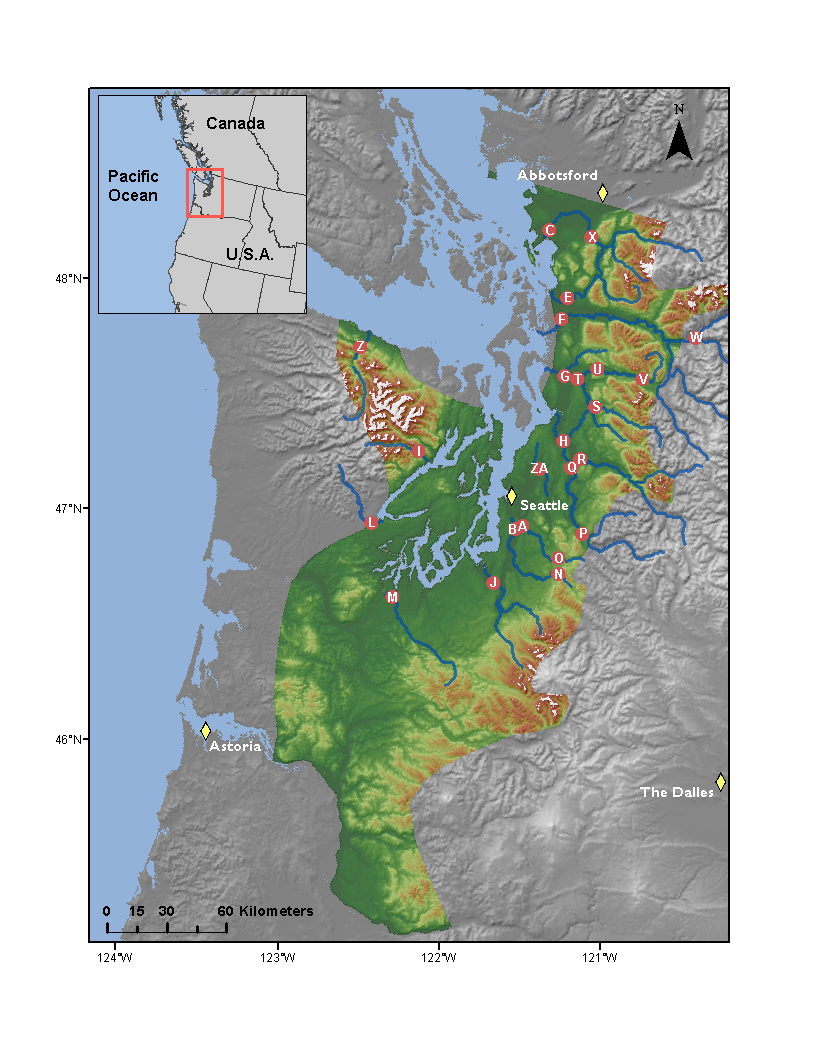
\includegraphics{figures/map/puget_sound_labeled.png}}
\textbf{Figure 1} Site locations (red points) in relation to combined Washington State Climate Divisions 3 and 4 (colored topography), the region across which climate data were aggregated. See Appendix C for site information.
\end{center}

Potential climatic predictors of T\textsubscript{water} and Q included mean and max T\textsubscript{air} (\degree C), total precipitation (cm), snowmelt (cm), and hydrological drought (Palmer Hydrological Drought Index), averaged by month across the response variable time series. All but snowmelt were available through the U.S. Climate Divisional Dataset, developed by the National Centers for Environmental Information (NCEI; \citealt{climateData}). We acquired climatic predictor data grouped by Washington State climate division, and all but two of our sites fell within divisions 3 (Puget Sound Lowland) and 4 (East Olympic/Cascade Foothills; see Fig. 1). We therefore aggregated these data by monthly mean across the two regions (after verifying their post-standardization similarity), resulting in a single dataset of four climatic predictor variables. A snowmelt time series was then added to this dataset, using monthly mean records from six SNOTEL sites (Bumping Ridge, Elbow Lake, Mount Crag, Park Creek Ridge, Stevens Pass, White Pass) listed by the USDA's Natural Resources Conservation Service; \citealt{snowData}. We calculated monthly snowmelt for each site as the absolute value of negative differences in cumulative snow water equivalent from each month to the next. The snowmelt time series was assigned zeros for any positive differences (accumulations).

\subsection*{Time series analysis}
Response time series (T\textsubscript{water} and Q) were modeled using dynamic factor analysis (DFA; \citealt{zuur2003estimating}), a multivariate technique that can be thought of as an analog to principal component analysis in the time domain. In DFA, response time series are fit with a linear combination of shared, random-walk trends (usually many fewer than the total number of response series), predictors (which can have unique effects on each response series), and random error. We chose DFA over a traditional multivariate state space approach for two reasons. First, it provides advantages in computational efficiency, as a small number of shared trends often adequately capture variation across dozens of responses, and at much lower parameter cost \citep{zuur2003dynamic}. Second, in terms of identifying what drives the shared trends, having fewer of them allows for greater inferential parsimony. Being a multivariate technique, DFA also provides an advantage over univariate alternatives in that covariance structure among responses can be specified and compared. All models were fit using maximum likelihood estimation by automatic differentiation, with Template Model Builder software \citep{kristensen2015tmb}, which we called using package TMB in R \citep{Rmanual,tmbPackage}.

DFA takes the following form:

\begin{equation}
    \textbf{x}_t = \textbf{x}_{t-1} + \textbf{w}_t\textrm{, where } \textbf{w}_t \sim \textrm{MVN}(0,\textbf{Q})
\end{equation}
\begin{equation}
    \textbf{y}_t = \textbf{Zx}_t + \textbf{Dd}_t + \textbf{v}_t\textrm{, where } \textbf{v}_t \sim \textrm{MVN}(0,\textbf{R})
\end{equation}
\begin{equation}
    \textbf{x}_0 \sim \textrm{MVN}(0,\bm{\Lambda})
\end{equation}

At time step {\it t}, the $m \times 1$ vector of shared trends (\textbf{x}) is a function of \textbf{x} in the previous step, plus normal error (\textbf{w}; $m\times 1$; Eq. 1). This is the definition of a random walk. The $n\times 1$ response vector (\textbf{y}) at time {\it t} is a function of the shared trends and their factor loadings (\textbf{Z}; $n\times m$), covariates (\textbf{d}; $q\times 1$) and their river-specific effects (\textbf{D}; $n\times q$), and a second normal error term (\textbf{v}; $n\times 1$; Eq. 2). \textbf{R} and \textbf{Q} are variance-covariance matrices of order m, and \textbf{Q} is set to identity for model identifiability \citep{harvey1990forecasting}. The initial state of the shared trend vector ($\bm{x}_0$) is multivariate-normally distributed with a mean of zero and a diagonal variance-covariance matrix with large variance (e.g. 5; Eq. 3). Response and predictor data were standardized to facilitate comparison of effect sizes and avoid error inflation.

Because we were interested in isolating the effects of climatic predictors on T\textsubscript{water} and Q, we used a fixed factor to account for recurring seasonal variation not related to the predictors, with one factor level for each month. This factor was incorporated into the covariate matrix (\textbf{d}). Thus, the coefficient in \textbf{D} relating, say, precipitation (predictor) and T\textsubscript{water} (response), represents the effect size of the former on the latter. In other words, it is the change in water temperature accompanying a unit change in precipitation across the whole time series. We call this relationship ``coupling.'' We were also interested in coupling by month for T\textsubscript{air}, which required that it be arranged as twelve separate, monthly time series. Concretely,

$$
\textbf{d} = \begin{blockarray}{cccccc}
& \textrm{Jan}_{1978} & \textrm{Feb}_{1978} & \textrm{Mar}_{1978} & \cdots & \textrm{Dec}_{2015} \\
\begin{block}{c(ccccc)}
    1 & 1 & 0 & 0 & \cdots & 0 \\
    2 & 0 & 1 & 0 & \cdots & 0 \\
    3 & 0 & 0 & 1 & \cdots & 0 \\
      & \vdots & \vdots & \vdots & \ddots & \vdots \\
    12 & 0 & 0 & 0 & \cdots & 1 \\
    13 & precip_1 & precip_2 & precip_3 & \cdots & precip_{456} \\
    14 & snowmelt_1 & snowmelt_2 & snowmelt_3 & \cdots & snowmelt_{456} \\
    15 & air_1 & 0 & 0 & \cdots & 0 \\
    16 & 0 & air_2 & 0 & \cdots & 0 \\
    17 & 0 & 0 & air_3 & \cdots & 0 \\
      & \vdots & \vdots & \vdots & \ddots & \vdots \\
    26 & 0 & 0 & 0 & \cdots & air_{456} \\
\end{block}
\end{blockarray}
$$

\noindent
is the covariate matrix structure necessary to account for seasonal variation of unknown origin (rows 1-12), and the effects of precipitation (row 13) and snowmelt (row 14), while also yielding the effect of T\textsubscript{air} by month (rows 15-26) on the response (\textbf{y}; Eq. 2). This is the covariate structure of the T\textsubscript{water} model we used for subsequent analyses, not including those described in Figure 5d-e, and Appendix B. The same form was used for the Q model.

Additional, non-seasonal variation due to unknown factors manifests in the shared trends, and a portion of any residual variation is absorbed by error matrix \textbf{v}. We fit models using four unique error structures (\textbf{R}), to allow for multiple suites of unknown drivers affecting rivers. We included shared variance with zero covariance, individual variance with zero covariance, shared variance with shared covariance, and individual variance with individual covariance. Details on these structures and their implications can be found in \citep{holmes2012marss}. The best models for T\textsubscript{water} and Q were determined via AIC. However, negligible likelihood improvements can be inflated when multiplied by thousands of data points, undermining common rules of thumb for admitting additional parameters under AIC \citep{burnham2003model}. Thus, we had reason to doubt that the ``most parsimonious'' model according to AIC alone was any better than a much simpler alternative. To manage this, we required that each additional trend, covariate, or seasonal structure improve the median coefficient of determination (R\textsuperscript{2}) by at least 1\% in order to justify accepting its attendant complexity.

\subsection*{Landscape predictors and post-hoc regression}
For post-hoc analyses, monitoring sites were separated into three classes based on relative areal coverage of perennial ice and/snow (hereinafter ``\% glaciation'') and mean elevation across their watersheds. The three classes are loosely based on the classification scheme and language of the Climate Impacts Group at the University of Washington \citep{mauger2015CIG}, and are here delineated according to Table 1.

% \begin{table}
\begin{center}
\textbf{Table 1} Watershed classification scheme
\end{center}
\begin{center}
\begin{tabular}{ |c|c|c|c| }
 \hline
 Classification & Abb. & Glaciation (\%) & Mean elev. (m) \\
 \hline
 Rain-dominated & RD & $< 0.7$ & $< 600$ \\
 Rain-and-snow & RS & $< 0.7$ & $\geq 600$ \\
 Snow-dominated & SD & $\geq 0.7$ & - \\
 \hline
\end{tabular}
\end{center}
% \end{table}

After model selection, climatic predictor effect sizes (\textbf{D}; Eq. 2) for each river were back-transformed to their original scales and regressed against landscape predictors in order to identify possible watershed-scale controls on coupling. To achieve this, we amassed an additional dataset of landscape features (Appendix C). These were collected individually for each of the watersheds corresponding to our 24 river sites, using the EPA's StreamCat (stream-catchment) data library \citep{hill2016stream} and the National Hydrography Dataset (NHDPlusV2; \citealt{mckay2012nhdplus}). Each site was mapped to an individual river reach, defined as a segment bounded on each end by a stream or river source, confluence, or mouth. The region contributing flow to this reach (its watershed) was then fetched, along with selected areal data, from the NHDPlusV2 database. Landscape attributes used as predictors were aggregated by watershed mean where applicable, and include elevation (m), total area (km\textsuperscript{2}), soil permeability (cm hr\textsuperscript{-1}), water table depth (cm), bedrock depth (cm), Base Flow Index (BFI; \%), runoff (mm mo\textsuperscript{-1}), percent perennial ice and snow coverage (National Land Cover Database [NLDC] 2006 and 2011 average), riparian population density (people km\textsuperscript{-2} within 100m of streams; 2010 census), riparian road density (km km\textsuperscript{-2}; 2010 census), and percent riparian urban land (NLCD 2011). Monitoring site elevation (m) and presence of upstream dams (as full/partial/no damming of upstream mainstem and major tributaries) were also included. Finally, we calculated area above 1000 m (as \% watershed area), mean slope (\% rise), and mean aspect (degree from true north) by delineating and summarizing watersheds from a digital elevation model in ArcMap v. 10.4 \citep{arcviewenvironmental}.

An additional set of post-hoc regressions was performed using factor loadings on shared trends (\textbf{Z}; Eq.2) as dependent variables, with landscape predictors again as independent variables. Loadings represent the degree to which each river's temperature fluctuates with the anonymous force driving the corresponding shared trend. A landscape feature that varies in proportion to these loadings is therefore likely to be a mediator of the anonymous force, if not the force itself. To facilitate inference by way of the shared trends, we made three simplifications to the model. We removed the monthly factor and the snowmelt predictor from the covariate matrix (\textbf{d}, rows 1-12 and 14), so that the trends would be free to express seasonal and elevational variation. Then, we limited the number of trends to between one and three, to avoid ``trend specialization.'' in other words, we optimized the trends for flexibility while concentrating their explanatory power. Additionally, we ordinated the landscape predictors with principal coordinates analysis (PCoA), as a way to conceptually ``group'' them by correlation. Data constrained to irregular, restricted ranges were scaled to [0-1] and arcsine-square-root transformed, along with all proportional data (The logit transform was avoided to prevent generation of infinite values.). All continuous data were then centered and scaled to unit variance before PCoA was performed. We used the Gower dissimilarity coefficient (Gower's distance) to account for association among both continuous and nominal variables \citep{gowerDist}.

\section*{Results}

Mean monthly temperature trends for the three river classes, aggregated across all 38 years of data, deviated by a minimum of 1.0\degree C in December, and a maximum of 3.9\degree C in July (Fig. 2). SD rivers remained approximately two degrees colder than their RS counterparts through mid-late summer, and 3-4 degrees colder than RD throughout spring and summer. RD rivers were consistently warmest throughout the year. In January, RS reached a minimum of 4.4\degree C, and did not significantly differ from SD (Student's t: $p<0.01, F=11.9$). RD only attained a minimum of 5.6\degree C. RS reached a peak summer temperature of 16.9\degree C in July, while RS and SD followed in August with peak temperatures of 15.5 and 13.5\degree C, respectively.

Meanwhile, the amplitude of T\textsubscript{air} oscillation exceeded that of any river class, dipping below T\textsubscript{water} in autumn to a minimum of 3.2\degree C in December, and rising above RS and SD in March to an August maximum of 17.4\degree C. T\textsubscript{air} did not overtake RD T\textsubscript{water} until August, by which time the latter had begun to decline.

% \begin{figure}[h!]
\begin{center}
% 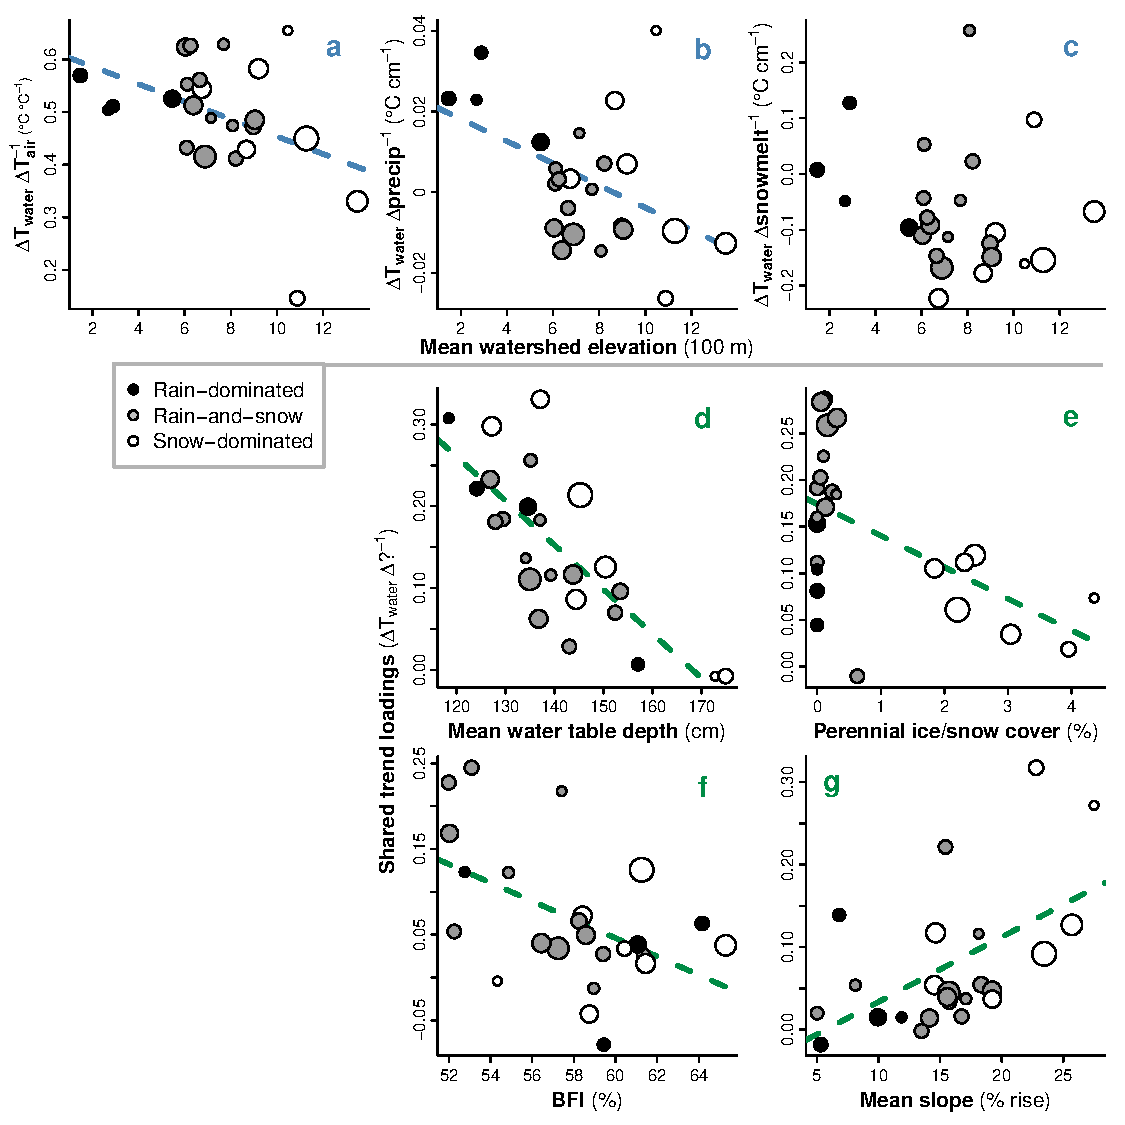
\includegraphics[width=\textwidth]{figures/16_temp_all_reg.pdf}
\resizebox{\textwidth}{!}{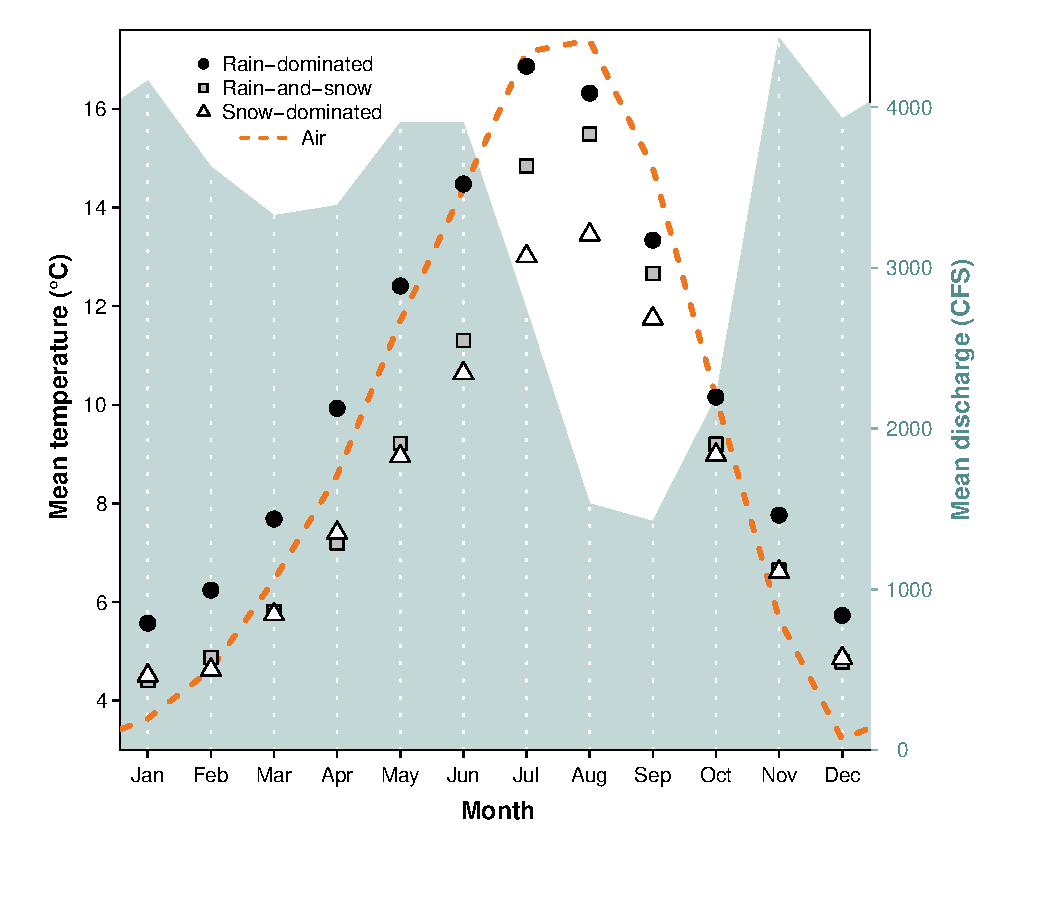
\includegraphics{figures/12_air_water_discharge.pdf}}
% \caption{Epipolar Geometry}
% \label{fig:air_water_disch}
\end{center}
% \end{figure}

\noindent
\textbf{Figure 2} Monthly mean T\textsubscript{water} by river class, and T\textsubscript{air} and Q across classes, from 1978 to 2015. All depicted series represent discrete data. %\setlength{\parskip}{6pt}
\\[\baselineskip]

The combined hydrograph of all rivers revealed two primary peaks, one beginning in late spring and the other extending from late autumn to early winter, with a prominent trough in late summer. Spring peak Q coincided noticeably with a separation in water temperature between SD and RS, while the summer trough coincided with separation of RD and T\textsubscript{air}. On average, November marked both the autumn peak in Q and the point at which T\textsubscript{air} fell below T\textsubscript{water}.

There was also an apparent divergence in slope between RD and all snow-influenced rivers, beginning in early spring and culminating in June. Between June and July, RS and SD saw a large jump in temperature, which coincided with the decline in snowmelt.

% \begin{tikzpicture}
%     \draw (0, 0) node[inner sep=0] {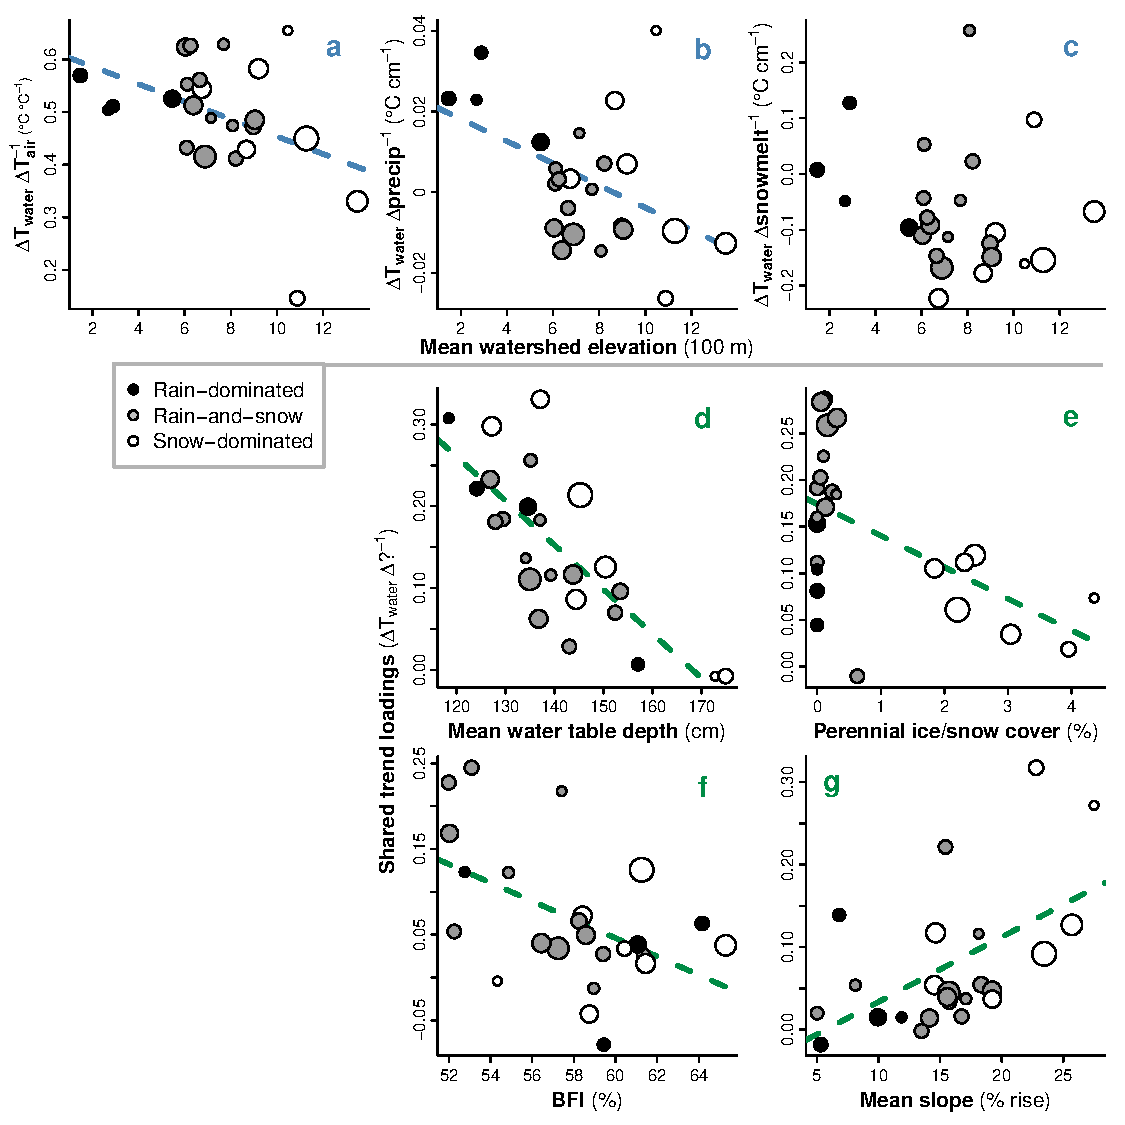
\includegraphics[width=\textwidth]{figures/16_temp_all_reg.pdf}};
%     \draw (-4.1, -2.1) node[text width=9.5em] {\normalsize \textbf{Figure 3} Relationships between watershed elevation and climatic effects on T\textsubscript{water} \textbf{(a-c)}, and other watershed predictors and factor loadings on shared trends \textbf{(d-g)}. Points are sized by watershed area. Regression lines indicate slopes significant at $\alpha=0.05$.};
% \end{tikzpicture}
\begin{center}
\resizebox{\textwidth}{!}{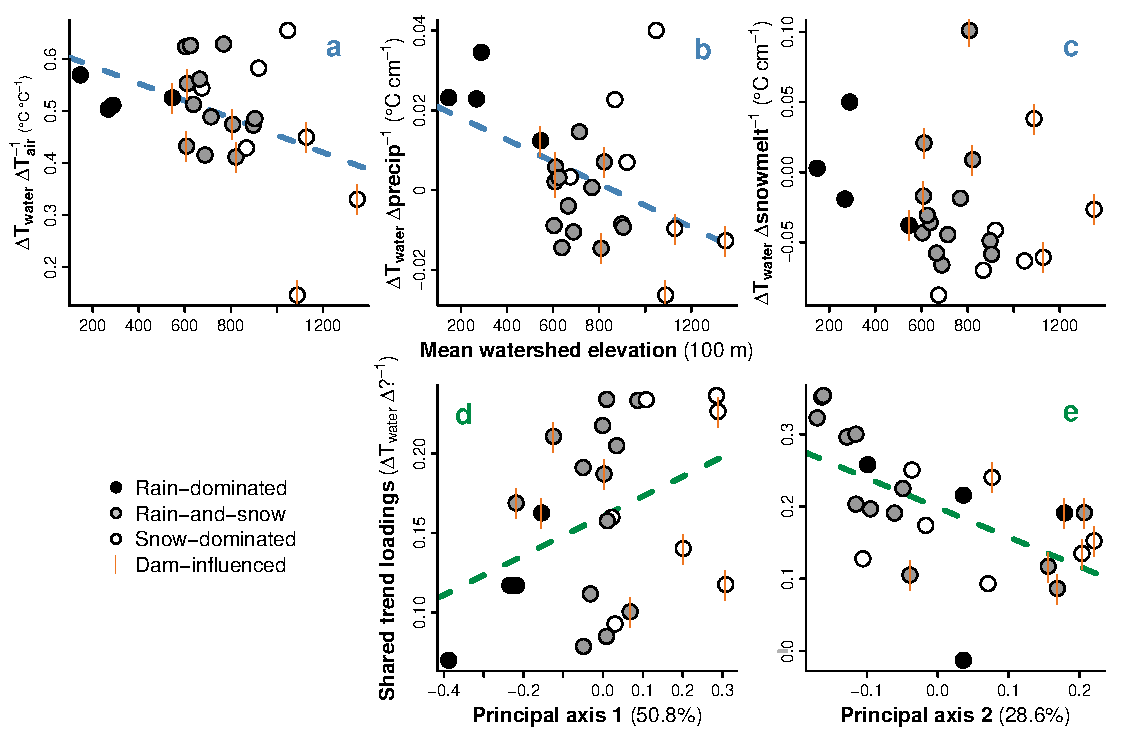
\includegraphics{figures/19_temp_simp_reg.pdf}}
% \textbf{Figure 3} Relationships between watershed elevation and climatic effects on T\textsubscript{water} \textbf{(a-c)}, and between watershed features and factor loadings on shared trends \textbf{(d-e)}. Regression lines indicate slopes significant at $\alpha=0.1$.
\resizebox{\textwidth}{!}{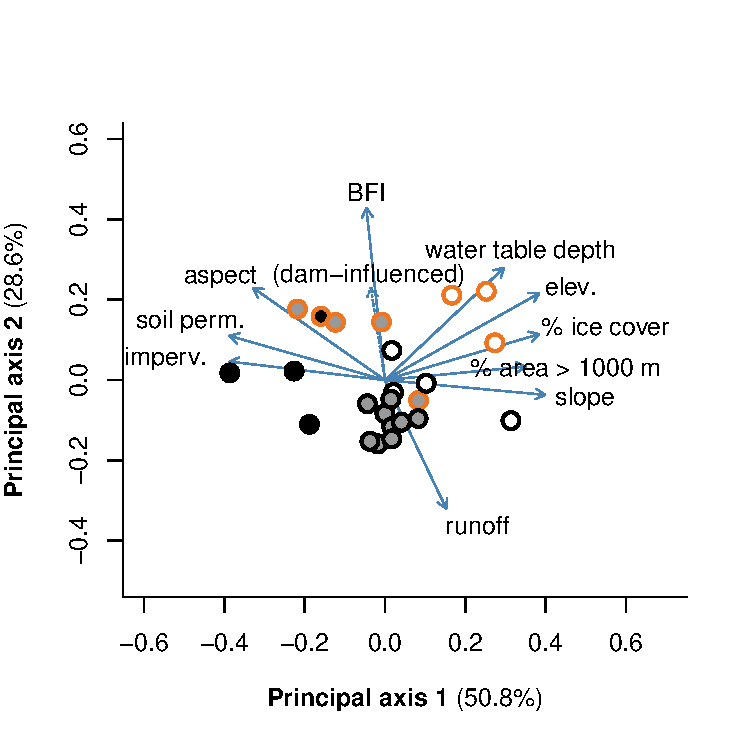
\includegraphics{figures/18_PCoA.pdf}}
\end{center}
\textbf{Figure 3} (a-c) Relationships between watershed elevation and climatic effects on T\textsubscript{water}, obtained from full model fit. (d-e) Relationships between watershed features and factor loadings on shared trends, from constrained model fit. Regression lines indicate slopes significant at $\alpha=0.1$. (f) Ordination of landscape predictors by principal coordinates analysis. Length and direction of arrows are proportional to loading of landscape predictors onto each principal axis of their variation.
\\[\baselineskip]

DFA results, aggregated across months and years for each site, revealed a trend toward reduced $\textrm{T}_{air}\rightarrow \textrm{T}_{water}$ coupling with increasing watershed elevation ($p=0.04, \textrm{mult.} R^2=0.18$; Fig. 3a). On average, a 1\degree C change in T\textsubscript{air} corresponded to a $0.53\pm 0.03$\degree C change in T\textsubscript{water} at RD, a $0.51\pm 0.08$\degree C change at RS, and a $0.45\pm 0.17$\degree C change at SD sites. A similar trend was observed with respect to $\textrm{precip}\rightarrow \textrm{T}_{water}$ coupling ($p=0.03, \textrm{mult.} R^2=0.21$; Fig. 3b), where a monthly change in total precipitation of 1 cm corresponded to a $0.02\pm 0.009$\degree C change in T\textsubscript{water} for RD, $-0.003\pm 0.009$\degree C for RS, and $0.004\pm 0.02$\degree C for SD. There was no evidence of coupling overall between snowmelt and T\textsubscript{water} (Fig. 3c), but this predictor was included in the most parsimonious DFA model selected via AIC and R\textsuperscript{2} (See Appendix A.). The strongest examples of $\textrm{T}_{air}\rightarrow \textrm{T}_{water}$ and $\textrm{precip}\rightarrow \textrm{T}_{water}$ coupling were observed in the Duckabush River, while the weakest examples are from the Elwha River. Both rivers drain glaciers of the Olympic Mountain Range, and both are SD. Among SD rivers, those influenced by dams appear to couple less strongly with T\textsubscript{air} and precip, but more so with snowmelt.

% In addition to the three climate predictors above, the best T\textsubscript{water} model also included five shared trends. Of these, four correlated significantly with at least one known watershed predictor. Figure 3 depicts the strongest correlated variables with each trend (insets d-e). These are, in arbitrary order, mean water table depth ($p<0.001, \textrm{mult.} R^2=0.60$; Fig. 3d), \% glaciation ($p<0.01, \textrm{mult.} R^2=0.30$; Fig. 3e), BFI ($p=0.01, \textrm{mult.} R^2=0.25$; Fig. 3f), and mean slope ($p<0.01, \textrm{mult.} R^2=0.29$; Fig. 3g). The fifth shared trend was not correlated with any variables in the watershed predictor dataset.
Factor loadings from a constrained, two-trend model each correlated with one of the two dominant, principal axes of variation across landscape predictors, determined by PCoA (Fig. 3f). The first principal axis was driven by mean watershed slope, snow (\% area > 1000 m) and ice, soil permeability, and other features that vary along elevational gradients, as well as mean elevation itself. Watershed's scores along this axis correlated with loadings from one trend, with marginal significance ($p=0.07, \textrm{mult.} R^2=0.14$; Fig. 3d). The second principal axis was driven by runoff, base flow, and upstream dams, and correlated with the other trend's loadings ($p<0.01, \textrm{mult.} R^2=0.35$; Fig. 3e). Combined, the first two principal axes accounted for 79.4\% of variation across landscape predictors.

\begin{center}
\resizebox{\textwidth}{!}{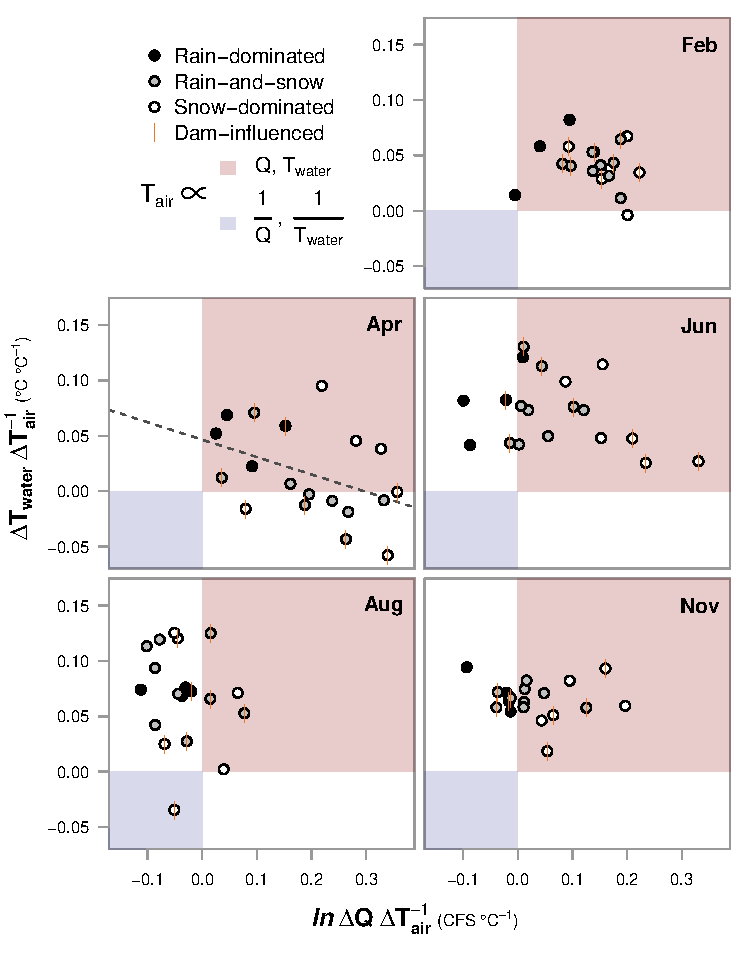
\includegraphics{figures/15_disch_vs_air_focal5.pdf}}
\end{center}
\textbf{Figure 4} Relationship between $\textrm{T}_{air}\rightarrow \textrm{T}_{water}$ and $\textrm{T}_{air}\rightarrow \textrm{Q}$. Both axes are expressed per 1\degree C change in $\textrm{T}_{air}$. The red quadrant designates proportionality between all three variables, the blue inverse proportionality between each response and $\textrm{T}_{air}$. Regression lines indicate slopes significant at $\alpha=0.05$.
\\[\baselineskip]

To examine possible sub-season interactions between T\textsubscript{air}, T\textsubscript{water} and Q, we performed an additional DFA with Q as the response. In both models, T\textsubscript{air} was allowed to have unique monthly effects. These effects, taken together, can be conceptualized in relation to the four quadrants of the Cartesian coordinate system (increasing clockwise from upper right; Fig. 4).

In mid-winter (exemplified by February), all river classes primarily occupy the first quadrant, signifying $\textrm{T}\textsubscript{air} \propto \textrm{T}\textsubscript{water}$ and $\textrm{T}\textsubscript{air} \propto \textrm{Q}$, where $\propto$ denotes proportionality. RD shows the weakest Q response. By spring, many RS and SD sites develop an inverse relationship between T\textsubscript{air} and T\textsubscript{water}, denoted $\textrm{T}\textsubscript{air} \propto \frac{1}{\textrm{T}\textsubscript{water}}$, while RD sites change little from their winter state. June and August see a procession of most sites into the near fourth quadrant, with SD trailing. This signifies $\textrm{T}\textsubscript{air} \propto \frac{1}{\textrm{Q}}$, though $\textrm{T}\textsubscript{air} \propto \textrm{T}\textsubscript{water}$. One stark exception is again the Elwha river, which occupies quadrant three. By autumn, RS and SD have begun progress back toward their winter states, led by SD. RD, meanwhile, remain essentially unmoved from summer.

Rivers influenced by dams do not appear to deviate appreciably from the rest in February, August, or November. However, SD rivers in April divide across the x-axis according to whether they are dammed. Those with dams exhibit $\textrm{T}\textsubscript{air} \propto \frac{1}{\textrm{T}\textsubscript{water}}$, while $\textrm{T}\textsubscript{air} \propto \textrm{T}\textsubscript{water}$ for those without. Similarly, in June, dammed SD rivers display stronger coupling between T\textsubscript{air} and Q than those without dams.

\section*{Discussion}

The effects of climate on T\textsubscript{water}, inferred through dynamic factor analysis, suggest that nearly all rivers included in our dataset were influenced strongly by air temperature, precipitation, and/or snowmelt across 38 years of monthly data (Fig. 3a-c). At most monitoring sites, T\textsubscript{water} closely tracked changes in T\textsubscript{air}, on average responding to increases and decreases with proportional movements of up to 66\% magnitude. However, some rivers only weakly tracked T\textsubscript{air}, and patterns in the intensity of this coupling relate primarily to changing landscape features along an elevational gradient (Fig. 3f). Glaciation and yearly snow burden are prominent among these, and for reasons of ecological and hydrological implication, the primary focus of the following discussion, along with the interacting role of dams.

Before any analysis, a ``buffering'' effect (the inverse of coupling) of ice on river temperature can be seen in the yearly patterns of T\textsubscript{water} relative to T\textsubscript{air} (Fig. 2). The aggregate hydrograph peaks due to snowmelt from April to June, at the same time that the trajectories of RS and SD (snow-influenced rivers) start to drop off relative to RD. After snowmelt begins to subside, RS and SD recover with a noticeable jump. For rivers that receive glacial runoff (SD), this buffering effect appears to remain into the summer months, guarding them from temperature rise when RS rivers instead approach the temperature of RD (Fig. 4). In an extreme case, the Elwha River was actually cooler in August during those years in which air temperature was higher, probably due to increased runoff from Carrie and Eel glaciers. The buffering effect of ice on river temperature is therefore two-fold, acting first on all snowmelt-influenced rivers through a cold-water pulse in spring, and then on a subset of those rivers throughout summer and autumn, by way of glacial runoff. For RD rivers, which receive little to no input from ice, summer temperature is entirely dictated by that of the surrounding air, and any rain falling through it.

Temperature buffering by snow and ice appears to be enhanced by the action of artificial impoundments. Eight sites on five rivers included in this study are (or were until 2014, in the case of the Elwha River) interrupted by dams or embankments that release stored water from the bases of their reservoirs. At 33 m, even the shallowest of these reservoirs is deep enough to stratify in summer, meaning released water would be delivered from the cold hypolimnion \citep{olden_hypoCold}. This certainly would have affected temperature readings for the Green, Elwha, Cedar and upper Skagit River sites, whose mainstems are or were dammed upstream of the sample location. The impact of damming on temperature readings at the Skokomish and the lower Skagit River sites should be lesser, as major, unobstructed river forks intercede between sample location and dam, resetting or partially resetting natural conditions \citep{stanford2001revisiting}. These sites are RS and SD, respectively, and both fall almost exactly on the regression line in Figure 4a. The upper Skagit site therefore occupies a middling space of $\textrm{T}_{air}\rightarrow \textrm{T}_{water}$ coupling between ``fully'' obstructed and unobstructed SD sites.

As for the unobstructed SD sites, they appear to oppose the trend exemplified overall. In particular, the Duckabush and Puyallup Rivers (upper white circles in Figs 3a, 3b, and 4-Apr.) noticeably break suit with the other SD sites in terms of $\textrm{T}_{air}\rightarrow \textrm{T}_{water}$ and $\textrm{precip.}\rightarrow \textrm{T}_{water}$, showing stronger relationships even than many of the RD rivers. Compared to all RS and RD rivers, and many SD, these stand out in terms of mean water table depth (Appendix C), suggesting they receive little influence from groundwater influx, which would otherwise serve to decouple $\textrm{T}_{air}$ and $\textrm{T}_{water}$. They also occupy smaller watersheds than most of the other SD rivers, which yield lower overall discharge and heat capacity, and thus greater susceptibility to temperature change \citep{caissie2006thermal}. There may be additional factors at work in the SD rivers that account for the surprisingly high coupling seen in some unobstructed SD rivers. Another potential candidate is watershed slope, which increases with elevation and affects T\textsubscript{water} by influencing residence time and evaporative cooling (via turbulence). High slope and elevation are also associated with lower-order tributaries, and thus lower heat capacity. 

The role of reservoirs in restructuring natural temperature coupling relationships is complex \citep{damsComplex,WarmingPostDam}, and here confounded with many additional variables. Omitting all obstructed sites from Figure 3a, it would appear that no trend exists, yet we believe such omission is unwarranted. If the presence of reservoirs negated the influence of other factors, there would be no separation between obstructed sites of different river classes. Furthermore, though cold, hypolimnetic outflow should be expected to buffer T\textsubscript{water} in summer, it alone cannot explain an {\it inverse} relationship between T\textsubscript{air} and T\textsubscript{water}. Instead, reservoirs may serve to enhance the decoupling of $\textrm{T}_{air}\rightarrow \textrm{T}_{water}$ and $\textrm{precip.}\rightarrow \textrm{T}_{water}$ brought on by snowmelt and glacial runoff, by selectively withholding warm water in their epilimnia and admitting cold water through their hypolimnia. Evidence for this phenomenon can be seen in the coupling of snowmelt and T\textsubscript{water}, which is generally greater in RS and SD sites downstream of obstructions (Fig. 3c). The Elwha River, which was cleared of its two dams between 2011 and 2014, will provide an excellent opportunity to compare each form of coupling with and without reservoirs, using the same dataset, once enough time has passed for signals to overcome inter-annual variability.

Though higher-elevation watersheds will always produce colder water, independent of the influence of ice and snow, it can be expected that RS and SD rivers will grow more similar to RD as regional temperatures warm and glaciers decline. That is to say, formerly reliably cold-water rivers and associated habitats may see increases in both summer and winter average temperatures, as well as higher variability from year to year. The Elwha in particular may slip from its current state of high resistance to seasonal climatic changes. We tested for changes in mean and variance of $\textrm{T}\textsubscript{air}\rightarrow \textrm{T}\textsubscript{water}$ and $\textrm{T}\textsubscript{air}\rightarrow \textrm{Q}$ coupling between 1978 and 2015, but did not detect any regular patterns (Appendix B).

In addition to the most parsimonious DFA, we fit a simplified model, designed to focus on what variation in T\textsubscript{water} could be explained by landscape predictors. The two trends of this model represent additional drivers responsible for structuring water temperature across some or all of the 24 sites included in the analysis. While the precise identities of these drivers cannot be obtained with certainty, they can be inferred through their relationships with predictor variables. In this way, we found elevation to be one of the dominant determinants of $\textrm{T}\textsubscript{air}\rightarrow \textrm{T}\textsubscript{water}$ and $\textrm{precip.}\rightarrow \textrm{T}\textsubscript{water}$, by driving variation in snow- and icemelt, soil permeability, and slope (Fig. 3f). Dams (reservoirs) and BFI (essentially groundwater contribution) were also major components of variation in temperature coupling, along with water table depth. Groundwater, being insulated from the air, maintains relatively constant temperatures throughout the year, particular if it is deep underground.

The relationship between climate and river temperature is further influenced by the interaction of discharge, and the fates of rivers in the Puget Sound watershed can be best understood by examining these factors in combination (Fig. 4). Whether rain-, both-, or snow-dominated, all rivers appear to take on RD characteristics in winter, when the effects of ice lay latent. As a result, warmer winters should on average yield warmer rivers and higher flow (less precipitation bound in ice). The critical differences between river classes play out in spring and summer, and it's during these months that future perturbations due to changing climate may be felt most acutely. For example, warmer Aprils on average produced colder water at 9 out of 15 RS and SD sites. Projected reductions in snowpack for the Pacific Northwest can therefore be expected to fundamentally alter the responses of currently snow-influenced rivers to yearly variation in spring temperature. In the longer term, changes can be expected for rivers that now receive the temperature-buffering effect of glacial runoff. Glaciers continue to decline across North America, with glacial ice across Western Canada projected to decline by 70\% from 2005 to 2100 \citep{clarke2015projected}.

\section*{Conclusion}

Temperature regimes across the rivers of the Puget Sound watershed are structured by a combination of climatic drivers at the regional scale, and geophysical drivers at watershed scales. In the absence of snow and ice, river temperature is closely coupled to that of the surrounding air, while discharge contributions from snowmelt and glacial runoff can dampen or even reverse this coupling in spring and summer, particularly where hypolimnetic-release reservoirs augment downstream cooling. In some cases, icemelt-influenced rivers exhibit stronger positive responses to climate patterns than their rain-driven counterparts. Our results suggest elevational variations in groundwater influx and total discharge may account for these patterns. However, while these factors and artificial reservoirs may influence the degree of coupling between climatic drivers and water temperature, only snow and ice can reverse it. Since 1978, such reversals have been widespread and commonplace, particularly during spring melt. Though we did not detect changes in this effect across historical observations, future reductions in snowpack and glacial mass are projected. Consequently, many rivers that now undergo the mildest seasonal temperature changes may be impacted most strongly.
\clearpage

\section*{Acknowledgements}
We thank Timothy Cline for the use of his TMB script, and Drs. Mark Scheuerell, Eric Ward, Eli Holmes, and Adrianne Smits for technical advice. Drs. Daniel Schindler and Michael Brett provided additional suggestions and guidance.

\bibliography{manuscript}
\bibliographystyle{apalike}
\clearpage

\section*{Appendix A}

\subsection*{Temperature DFA output and diagnostics}
The process of selecting the best T\textsubscript{water} and discharge models involved four climate covariates (air temperature, precipitation, snowmelt, and hydrological drought), between 1 and 15 shared trends, four within-and-among-site error structures (see methods), and two expressions of unknown seasonal variation (fixed monthly factors and Fourier series). The most parsimonious models were selected using the Akaike Information Criterion (AIC) in tandem with R\textsuperscript{2} (required increase of 1\% for each additional parameter), and in each case included air temperature, precipitation, and snowmelt as covariates. The T\textsubscript{water} model also included five shared trends and an independent and unequally distributed error structure among rivers (i.e. diagonal and unequal variance-covariance matrix). The discharge model (not shown) included six trends. All subsequent plots relate to the T\textsubscript{water} model, and alphabetic names correspond to sampling sites (Fig 1).

\begin{center}
\resizebox{\textwidth}{!}{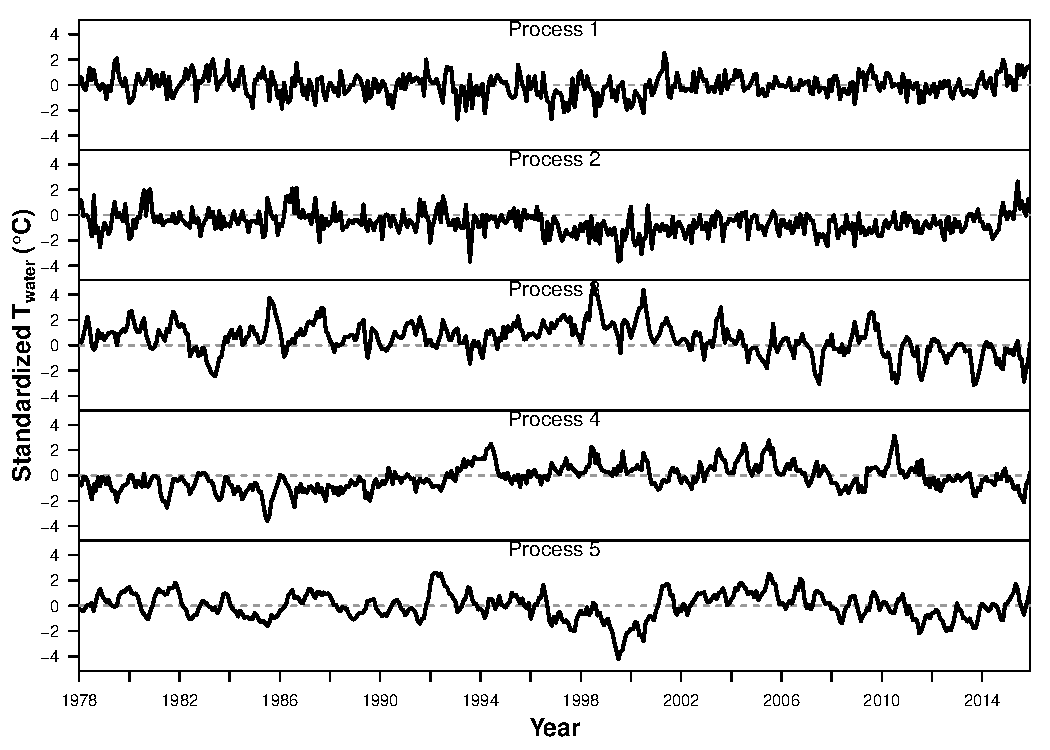
\includegraphics{figures/diagnostic_plots/01_trends.pdf}}
\end{center}
\textbf{Figure A1} Shared trends.

\begin{center}
\resizebox{\textwidth}{!}{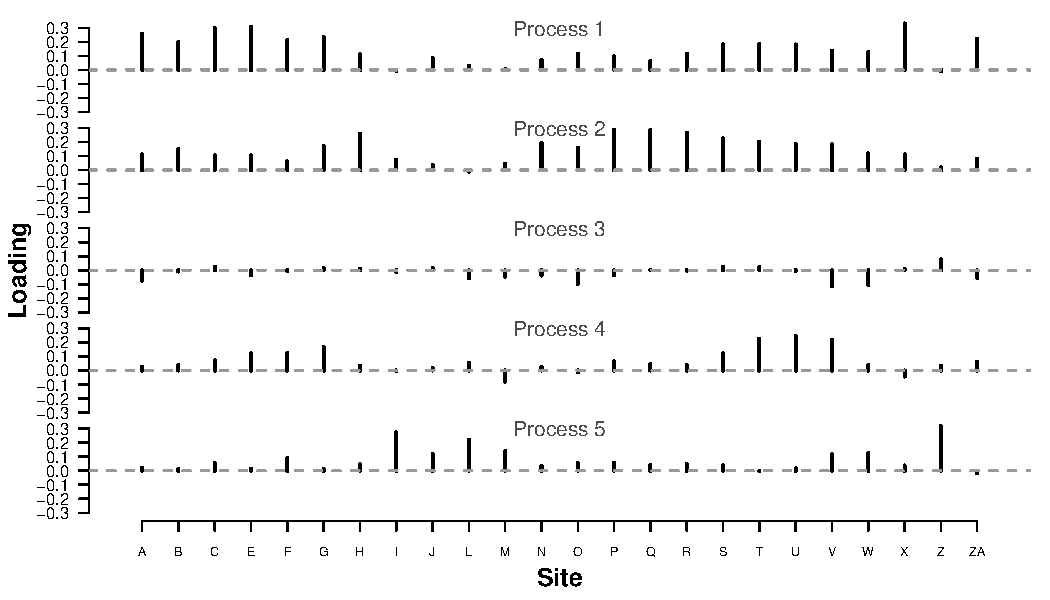
\includegraphics{figures/diagnostic_plots/02_loadings.pdf}}
\end{center}
\textbf{Figure A2} Factor loadings on shared trends.

\begin{center}
% \resizebox{\textwidth}{!}{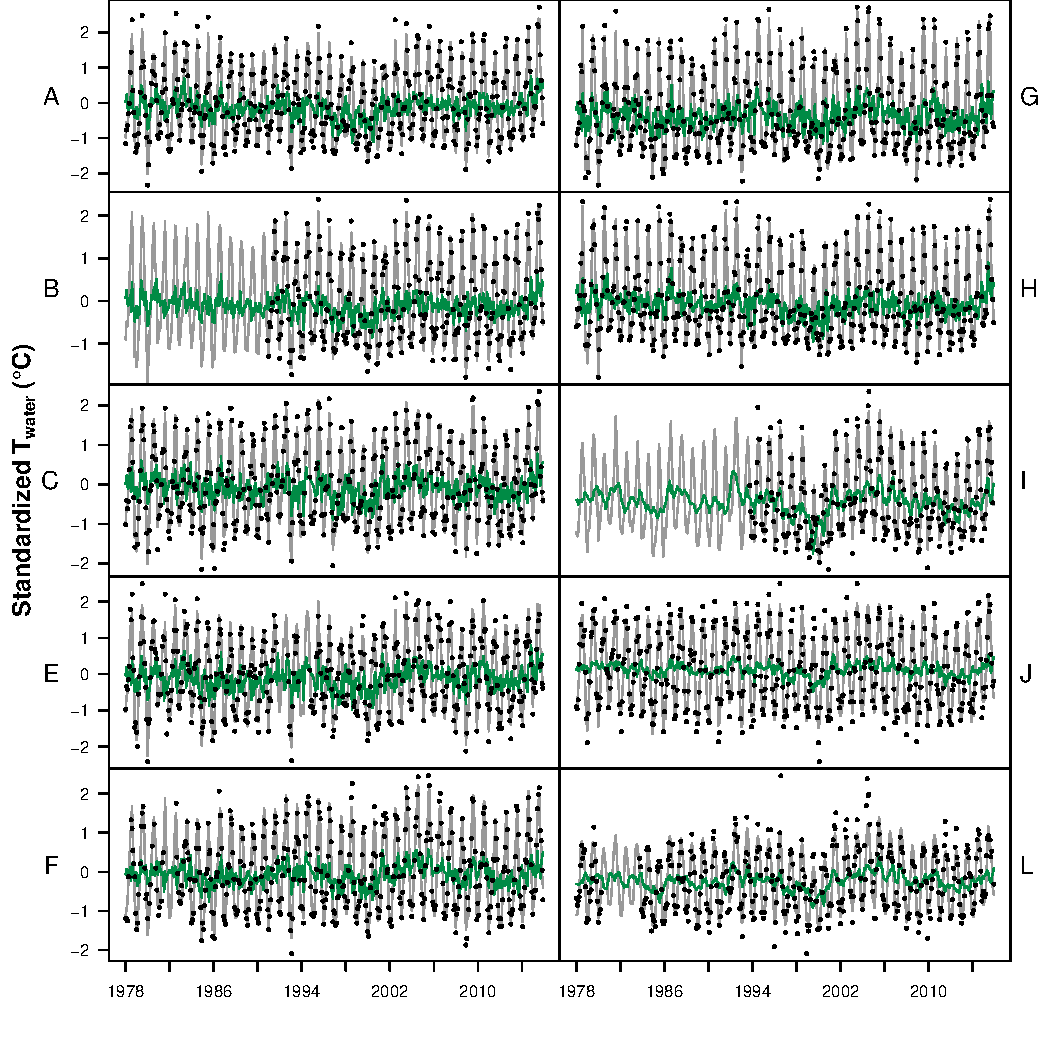
\includegraphics{figures/diagnostic_plots/03_fits.pdf}}
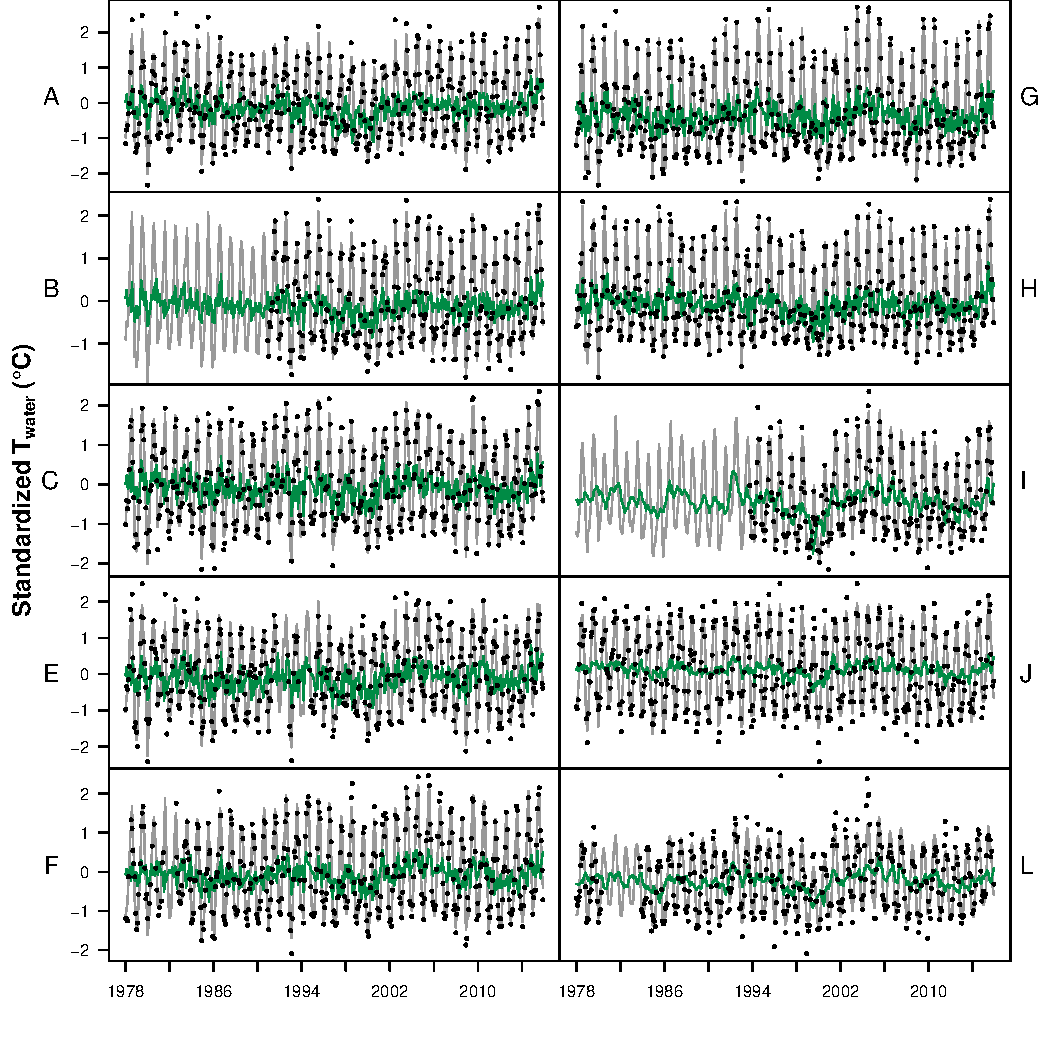
\includepdf[pages={1-},scale=0.75]{figures/diagnostic_plots/03_fits.pdf}
\end{center}
\textbf{Figure A3} Model fits (gray line = overall fit; green line = trends-only fit, points = data).

\begin{center}
% \resizebox{\textwidth}{!}{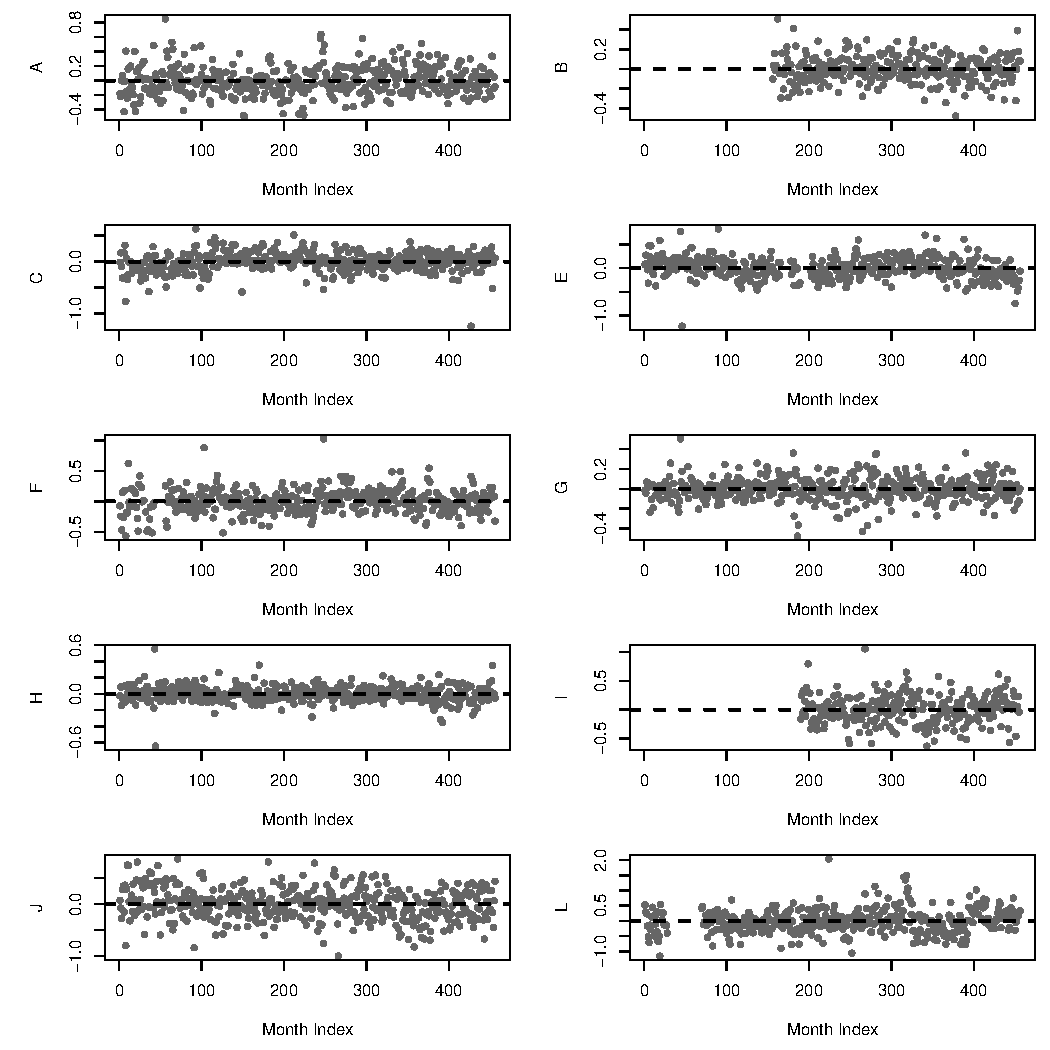
\includegraphics{figures/diagnostic_plots/04_residuals.pdf}}
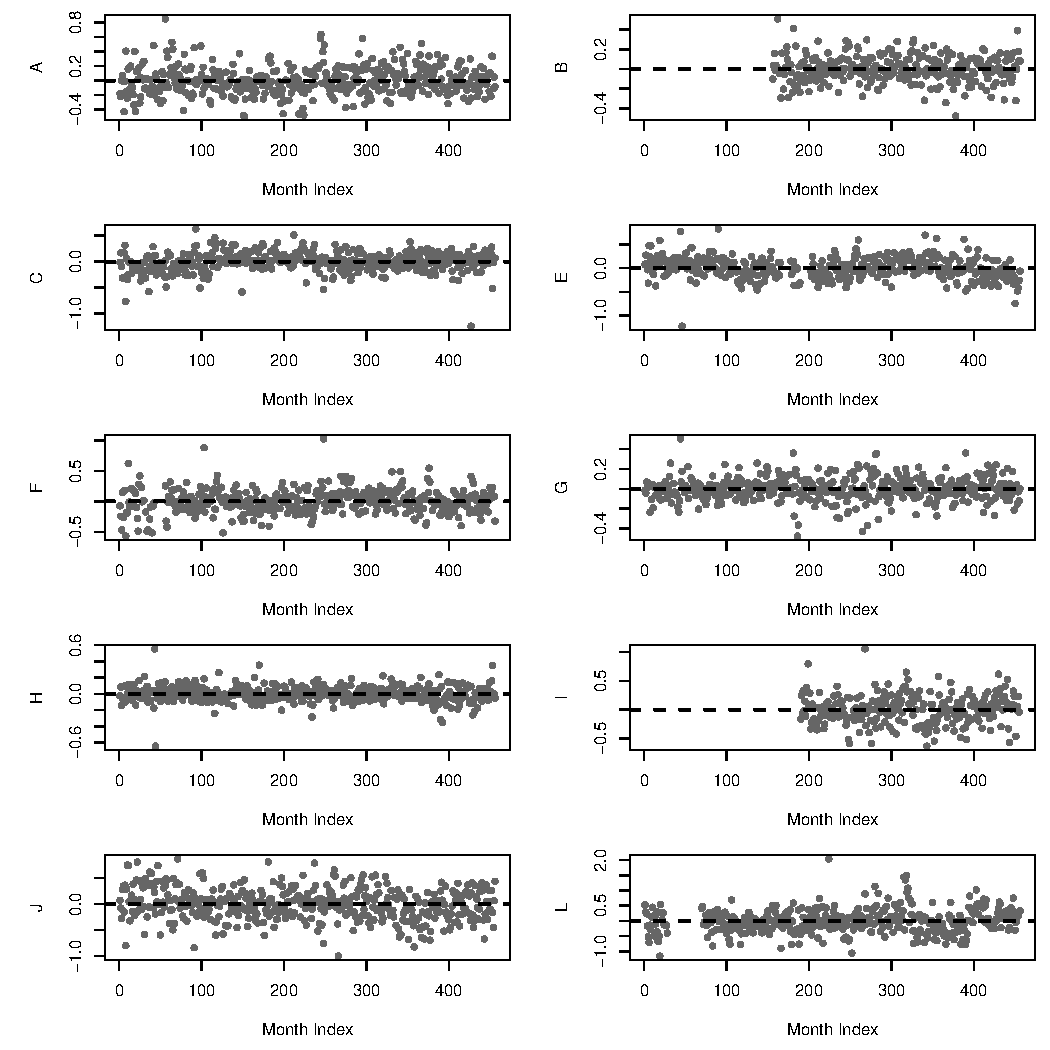
\includepdf[pages={1-},scale=0.75]{figures/diagnostic_plots/04_residuals.pdf}
\end{center}
\textbf{Figure A4} Residuals.

\begin{center}
% \resizebox{\textwidth}{!}{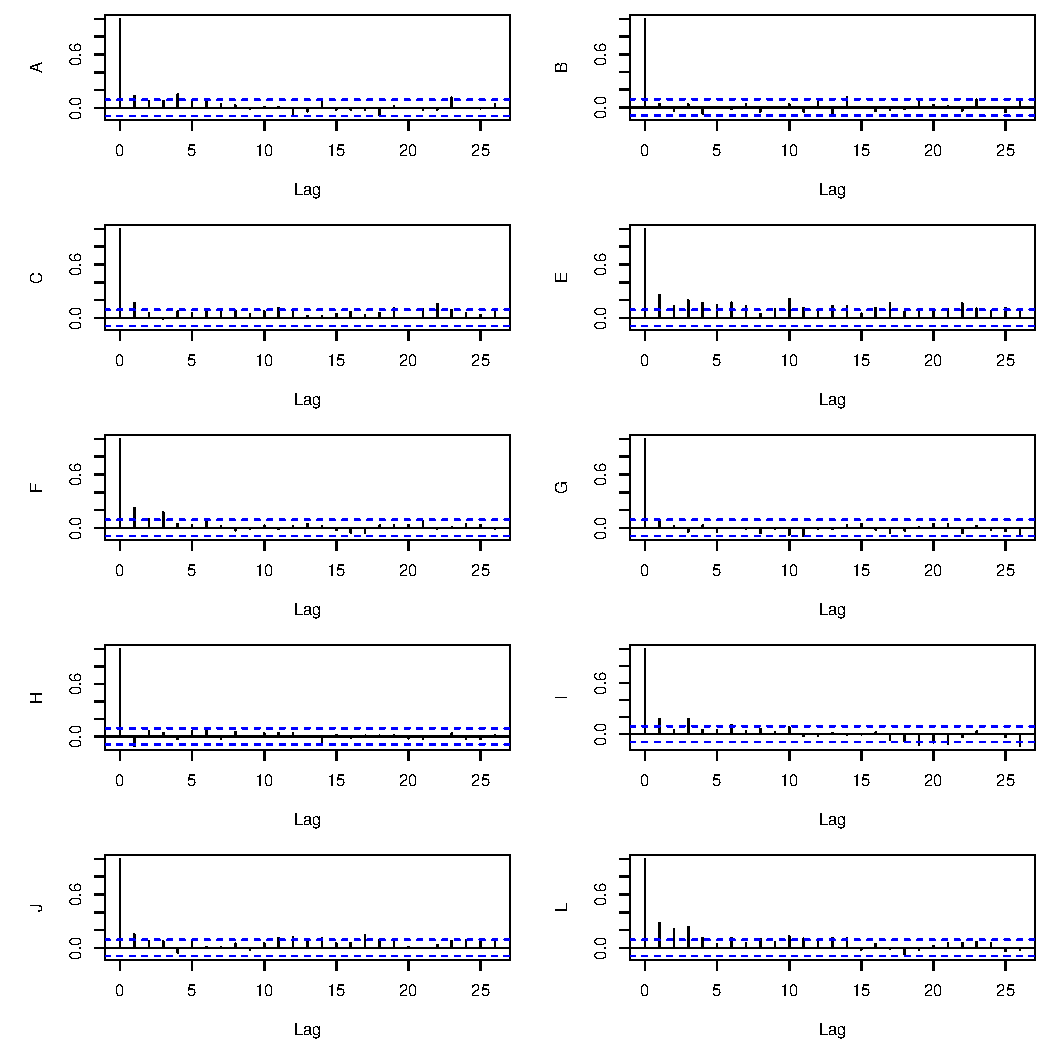
\includegraphics{figures/diagnostic_plots/05_acf.pdf}}
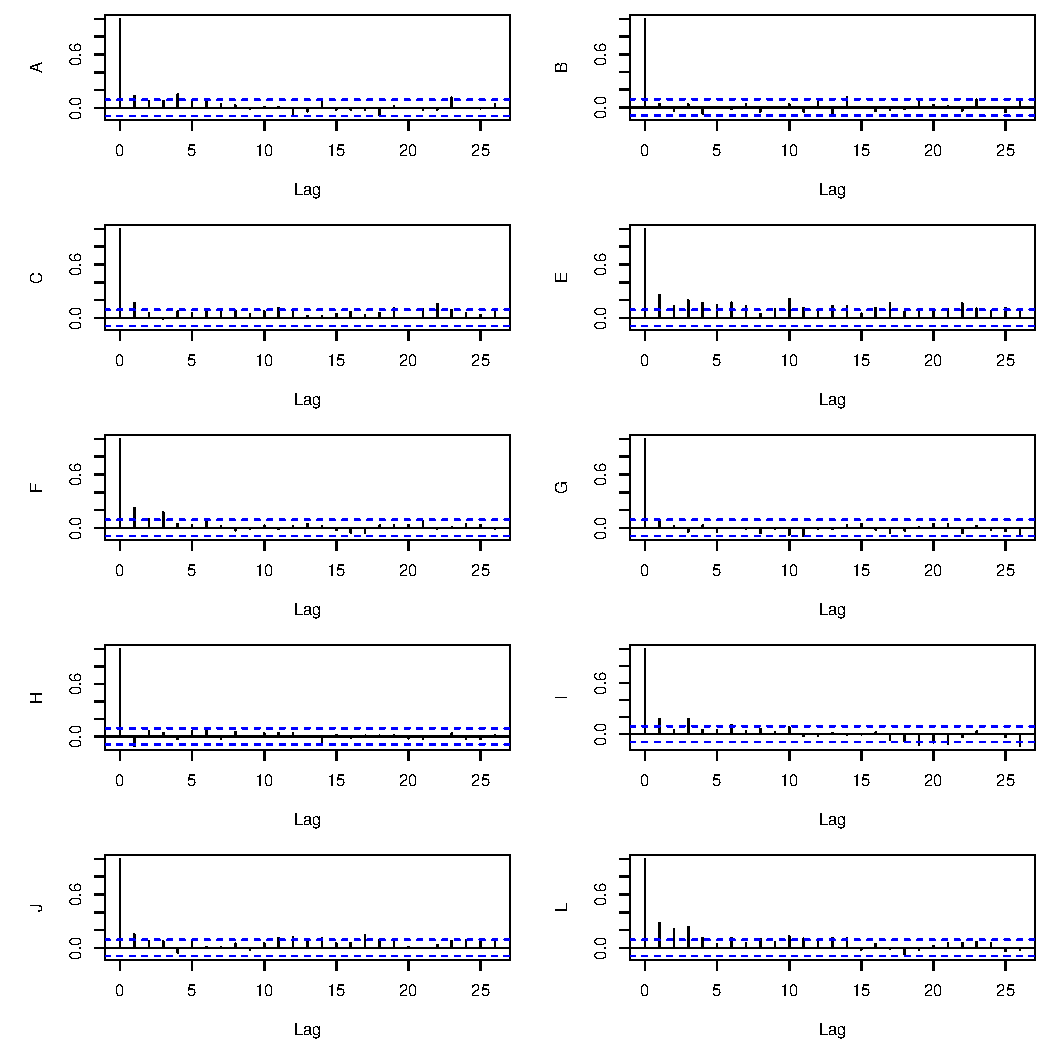
\includepdf[pages={1-},scale=0.75]{figures/diagnostic_plots/05_acf.pdf}
\end{center}
\textbf{Figure A5} Autocovariance function (ACF).

\begin{center}
\resizebox{\textwidth}{!}{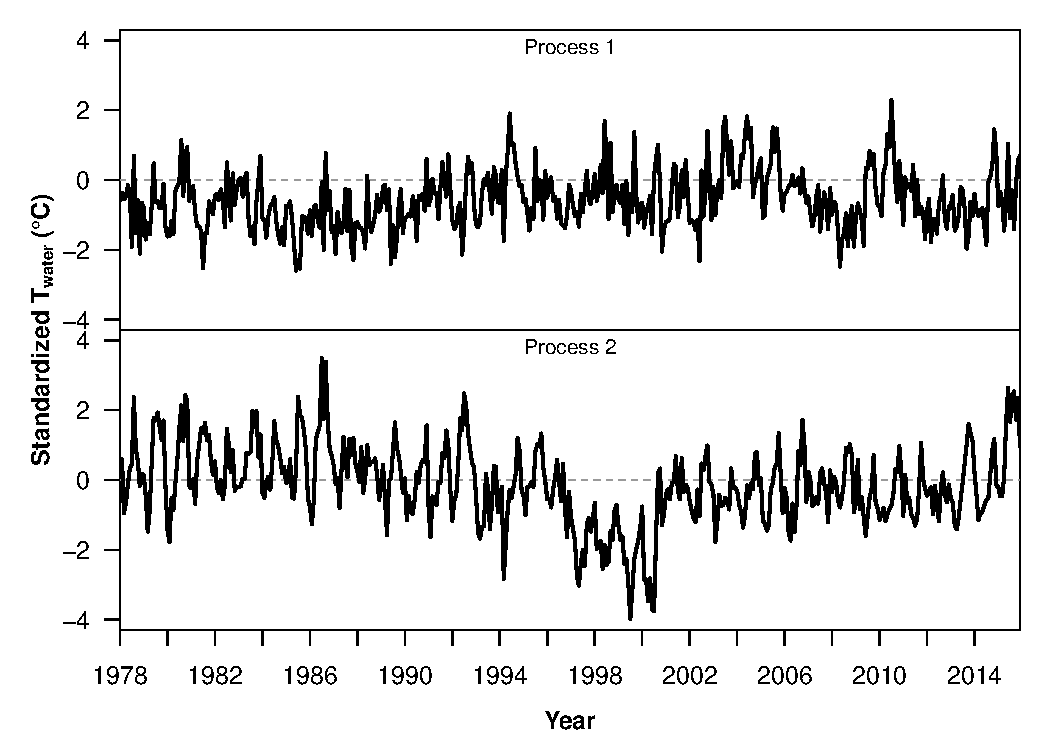
\includegraphics{figures/diagnostic_plots/01_trends_simp.pdf}}
\end{center}
\textbf{Figure A6} Shared trends from simplified model (no seasonal fixed factor, no snowmelt predictor)

\begin{center}
\resizebox{\textwidth}{!}{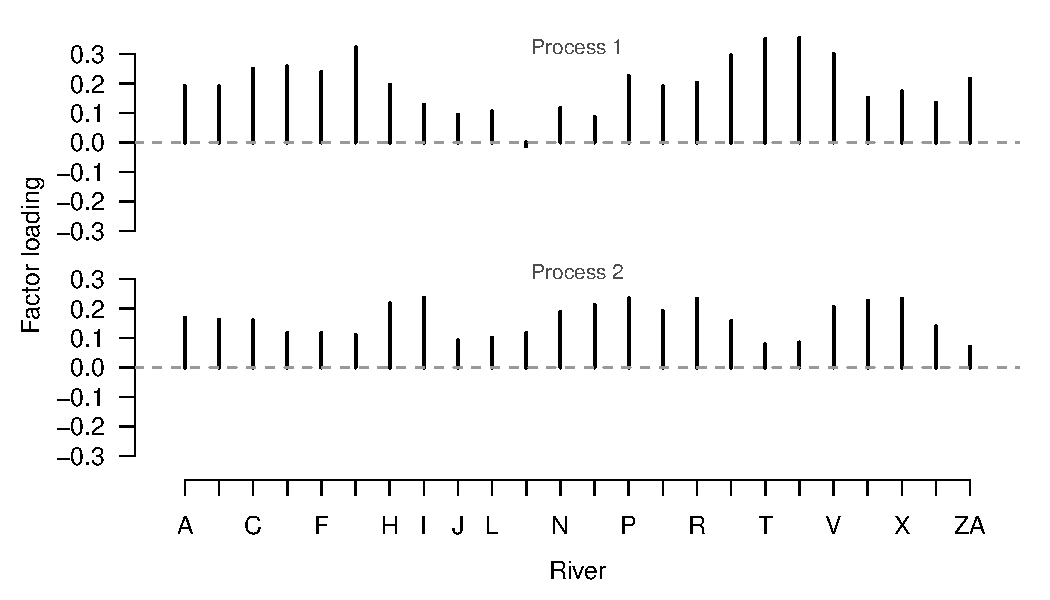
\includegraphics{figures/diagnostic_plots/02_loadings_simp.pdf}}
\end{center}
\textbf{Figure A7} Factor loadings from simplified model (no seasonal fixed factor, no snowmelt predictor)

\clearpage

\section*{Appendix B}

\subsection*{Testing for change in coupling over time}

We used an additional DFA model to test for changes in $T_{air}\rightarrow T_{water}$ coupling over time, by dividing the 1978-2015 time series into 5 intervals and comparing central tendency and variance of effect sizes for each interval. Figures B1-B3 show mean effect size for each river.

To approximate estimates of variability over time, we performed the same analysis within a Bayesian framework, and obtained uncertainty estimates from the credible intervals of the effect size posteriors. This approach yielded no trends in variation over time, and is not visualized here. For Bayesian analyses, we used R package ``statss'' \citep{eric_ward_2017_375646}.

\begin{center}
\resizebox{\textwidth}{!}{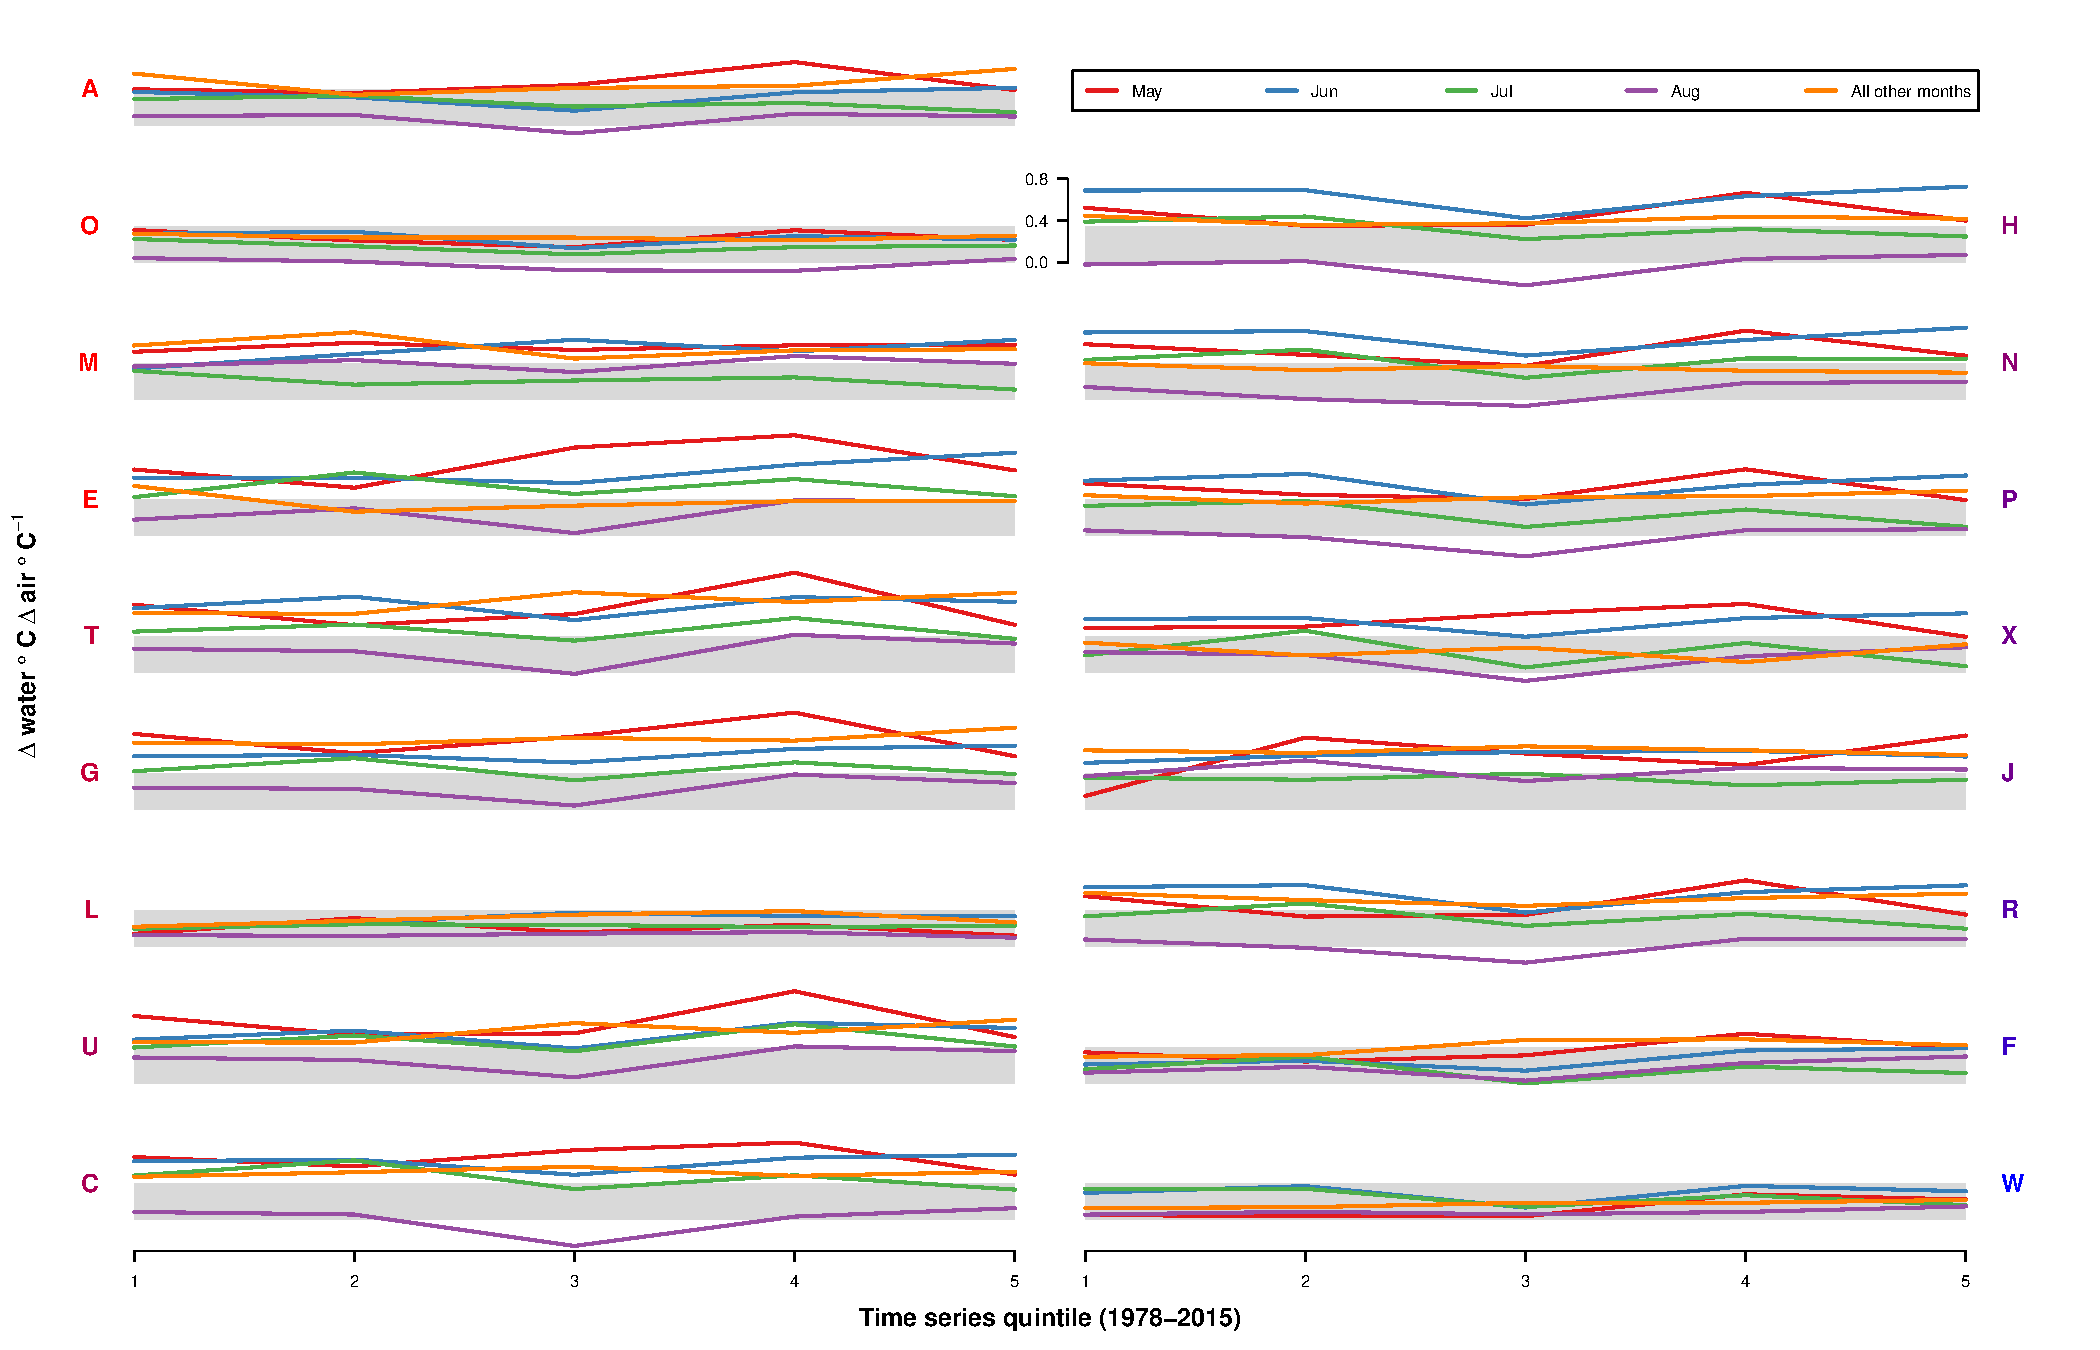
\includegraphics{figures/05a_temp_effSize_byMonth_acrossTime_may-aug.pdf}}
\end{center}
\textbf{Figure B1} Mean $T_{air}\rightarrow T_{water}$ coupling over time. Each plot corresponds to an individual site. Y-label colors represent mean watershed elevation (bluer=higher).

\begin{center}
\resizebox{\textwidth}{!}{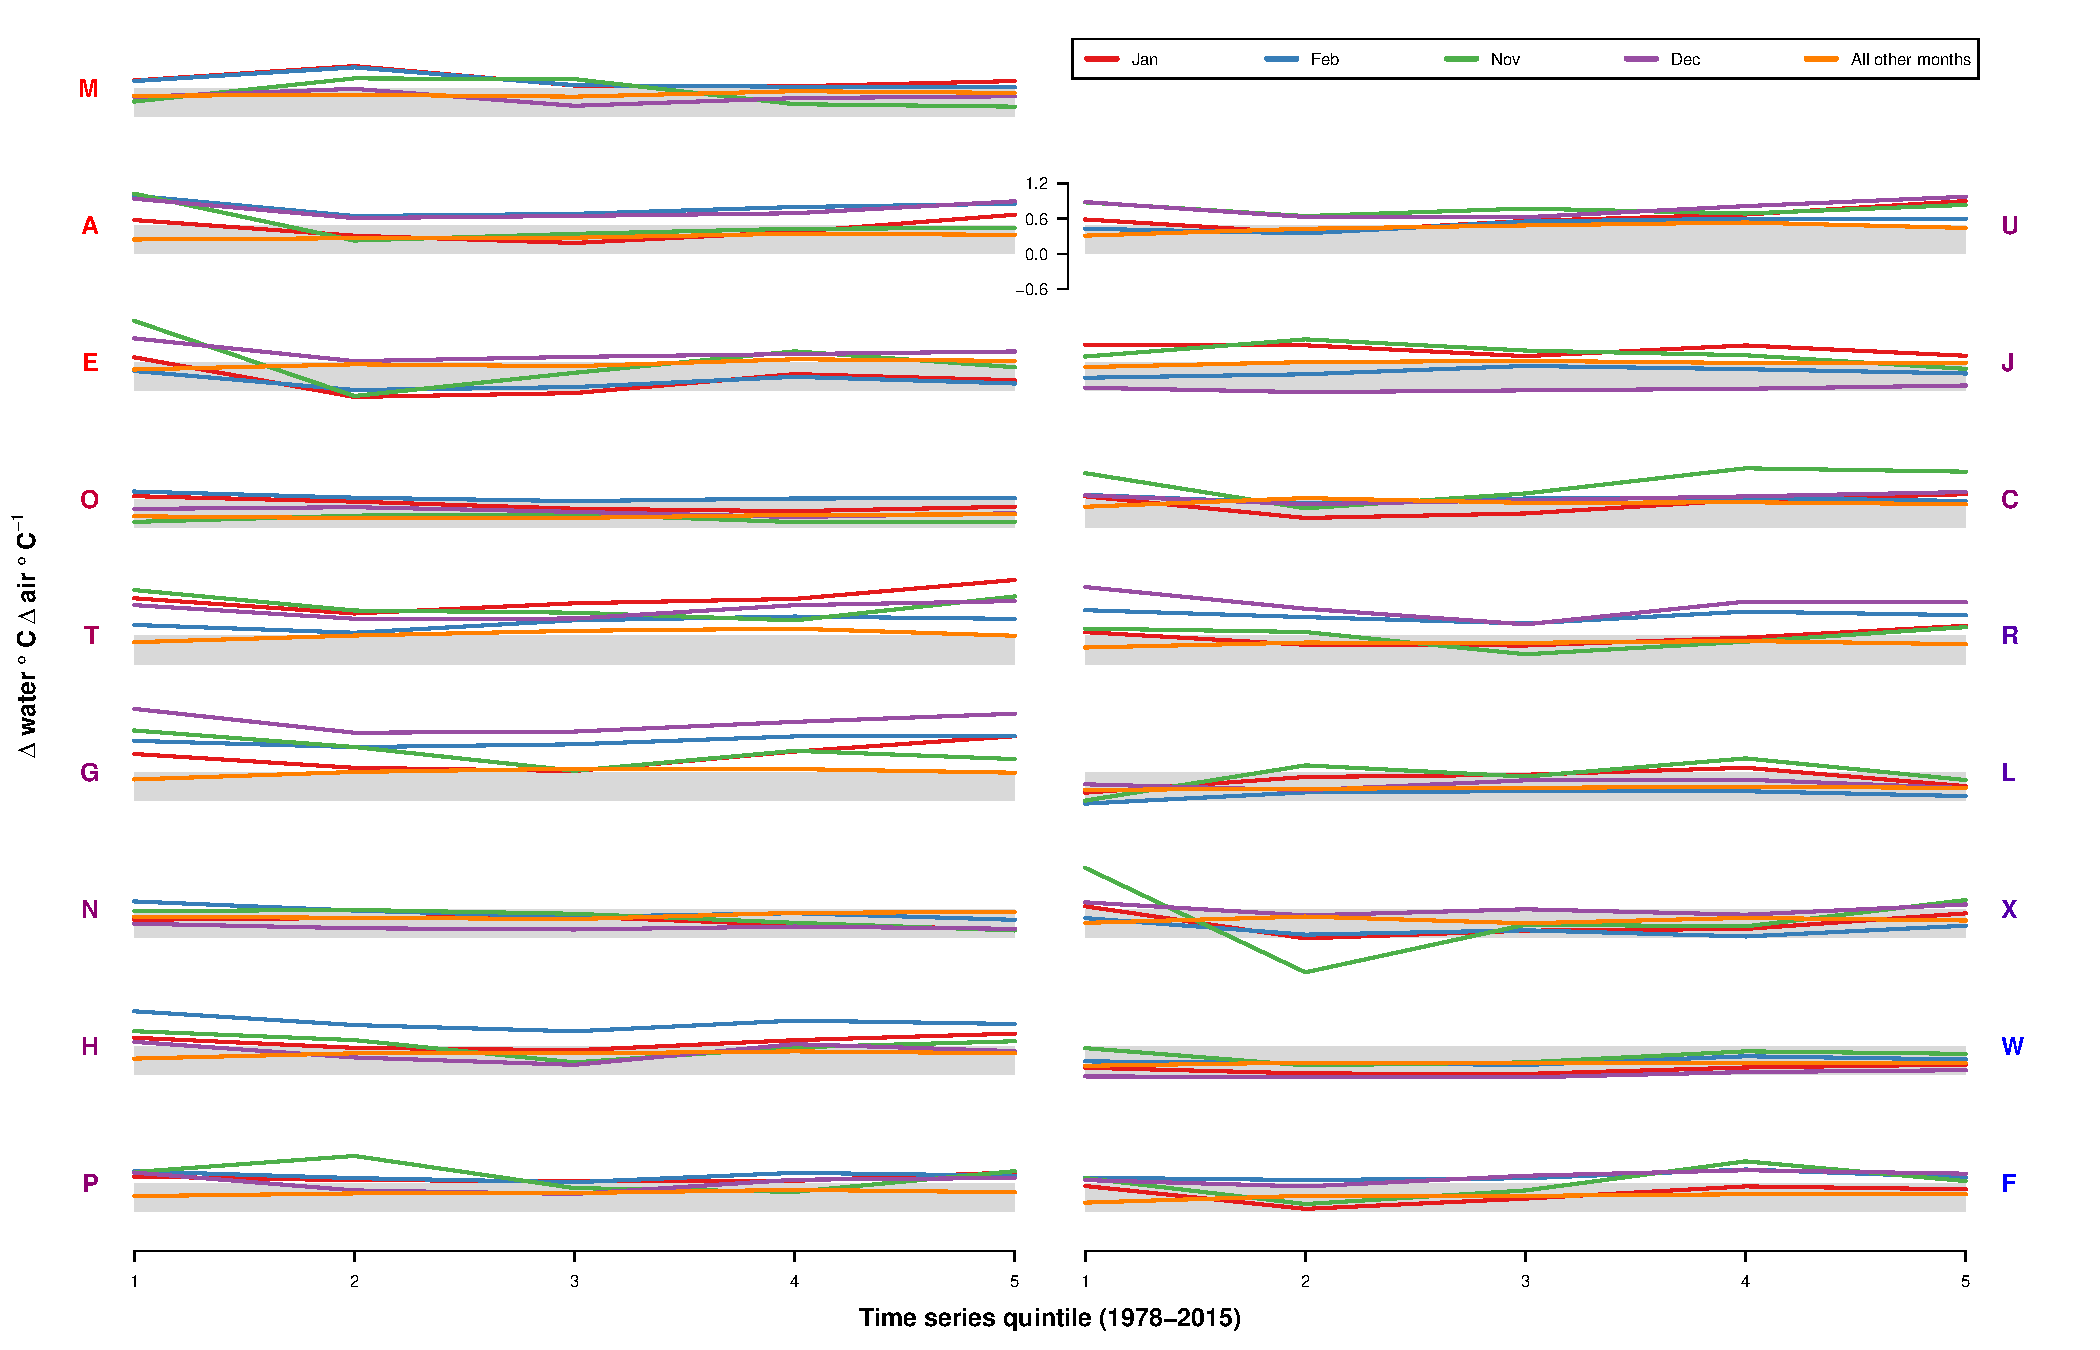
\includegraphics{figures/05b_temp_effSize_byMonth_acrossTime_nov-feb.pdf}}
\end{center}
\textbf{Figure B2} Mean $T_{air}\rightarrow T_{water}$ coupling over time. Each plot corresponds to an individual site. Y-label colors represent mean watershed elevation (bluer=higher).

\begin{center}
\resizebox{\textwidth}{!}{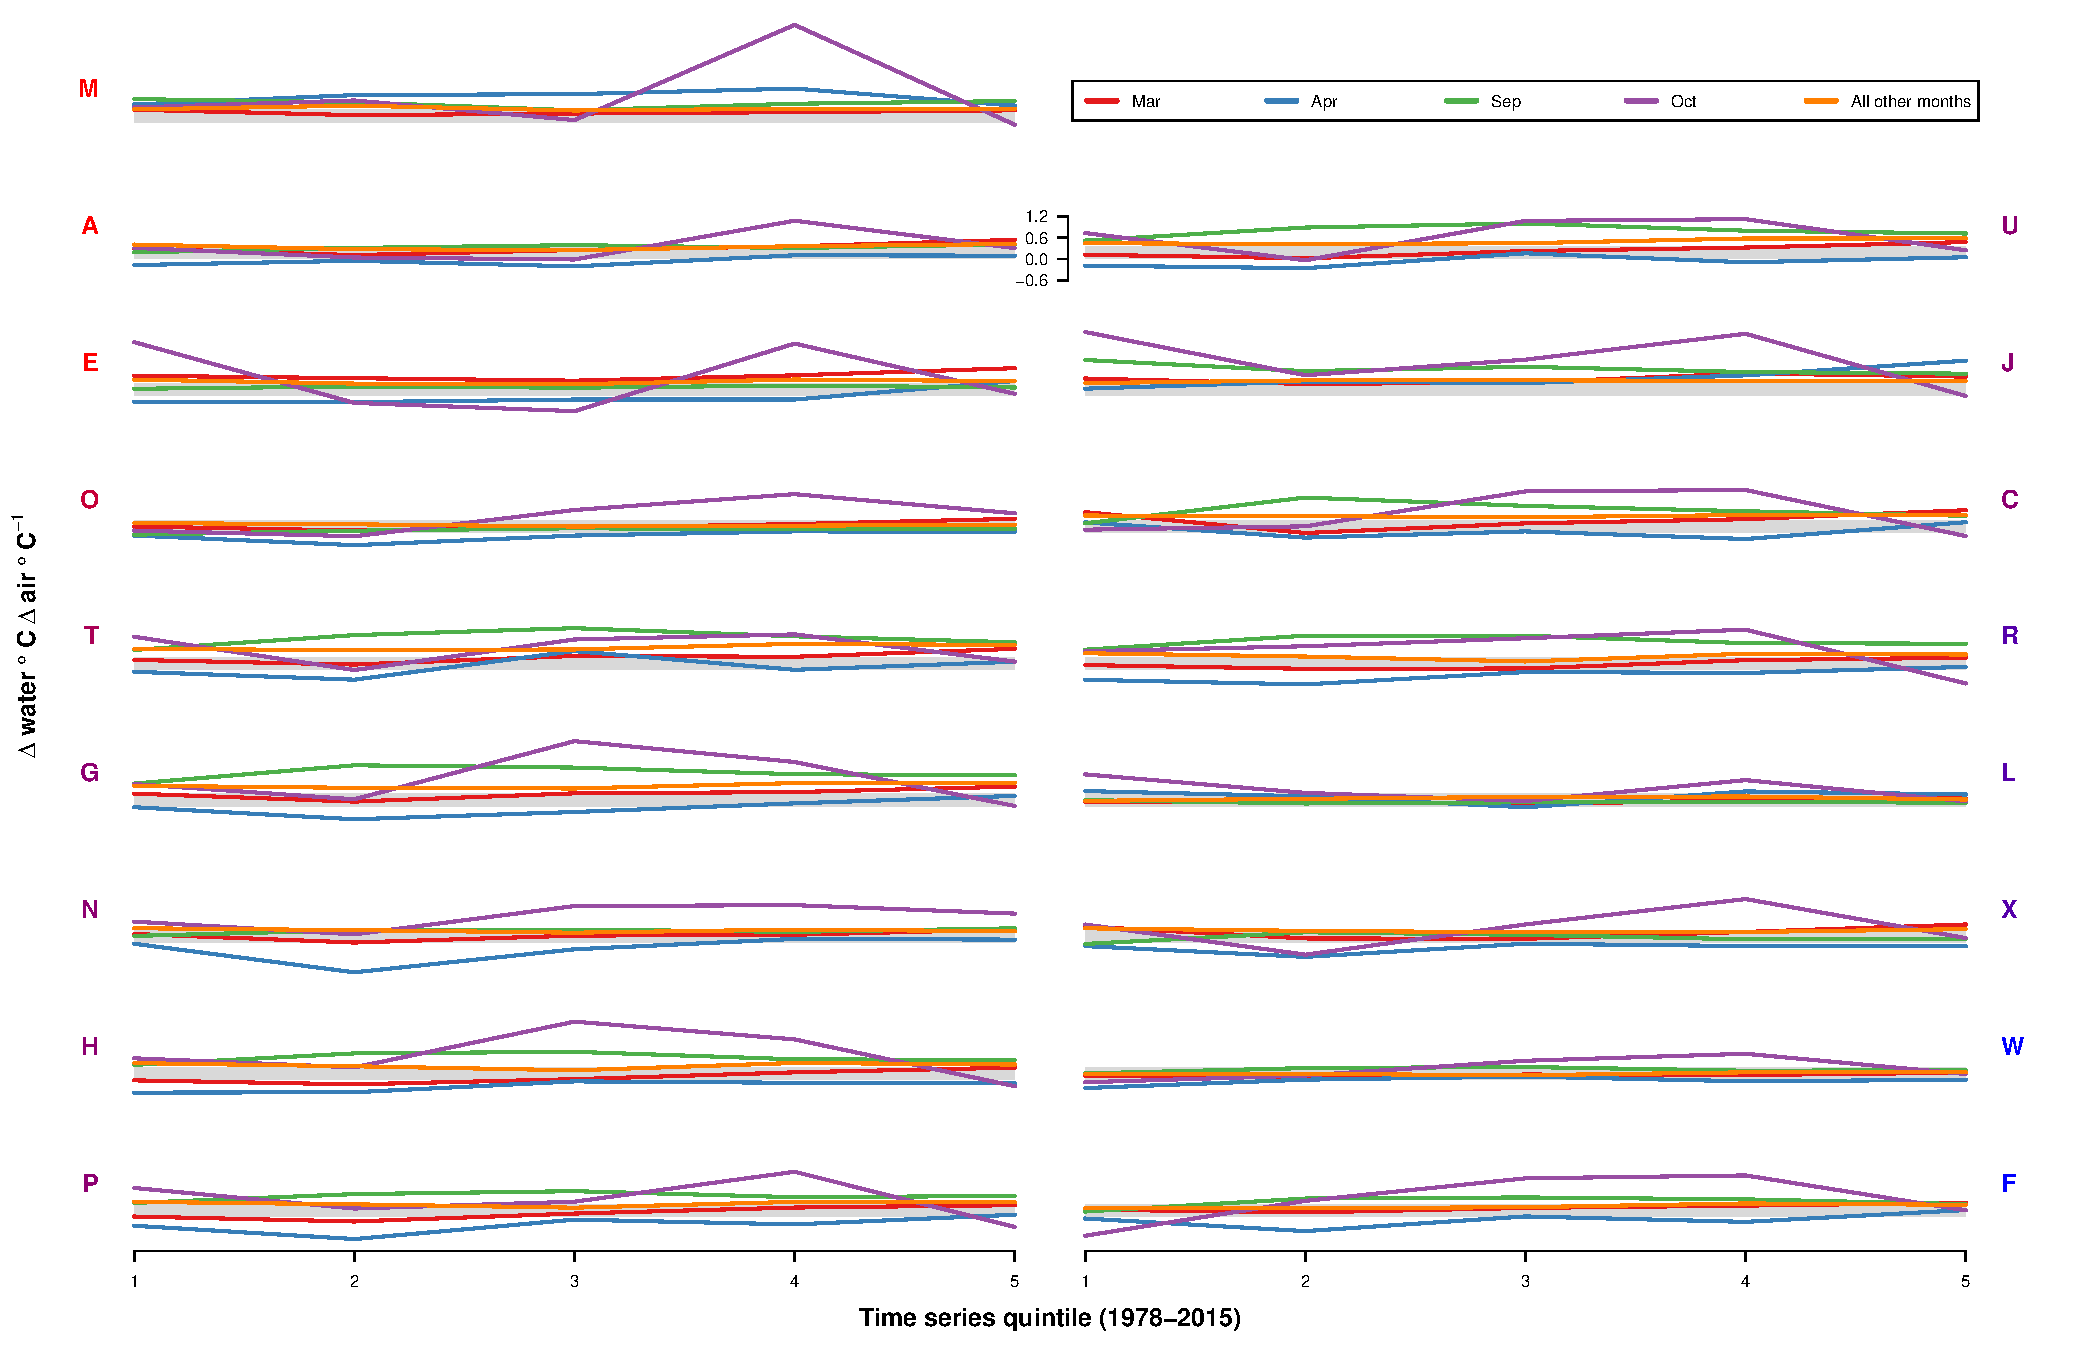
\includegraphics{figures/05c_temp_effSize_byMonth_acrossTime_MASO.pdf}}
\end{center}
\textbf{Figure B3} Mean $T_{air}\rightarrow T_{water}$ coupling over time. Each plot corresponds to an individual site. Y-label colors represent mean watershed elevation (bluer=higher).

\section*{Appendix C}

\textbf{Table C1}.
\begin{landscape}
\csvautolongtable[respect all]{table_C1a.csv}
\clearpage
\csvautolongtable[respect all]{table_C1b.csv}
% \csvautolongtable[respect all, tabular=|l|c|c|c|c|c|c|c|c|c|c|c|]{table_C1b.csv}
\end{landscape}

\end{document}
